\documentclass[aspectratio=43,8pt]{beamer}
\usepackage[utf8]{inputenc}
\usepackage{multicol}
\usepackage{hyperref}
\usepackage{graphicx}
\usepackage{babel}[french]
\hypersetup{
    colorlinks=true,
    urlcolor=blue,
    pdfborder={0 0 0},
}

\title{On Demand Buffer (ODB) - Resultats Obtenus}
\author[Brelot]{Julien Brelot}
\date{ \today}

\usetheme{material}
\useLightTheme
\usePrimaryGreen
\useAccentCyan

\setbeamertemplate{footline}[text line]{%
  \hfill%
  \insertframenumber\,/\,\inserttotalframenumber
}

\begin{document}

\begin{frame}
\titlepage
\end{frame}

\begin{frame}{Tests effectués}
    \begin{card}

        Un test de stress a été effectué 3 serveurs nginx sur 3 noeuds grid-5000 différents.
        Les 3 noeuds ont chacun 1 serveur nginx avec 1 worker.
        Le front-end et le serveur intermédiaire sont 2 serveurs proxy.
        Le back-end est un serveur http qui fournit les fichiers au proxy intermédiaire.
        Le proxy_buffering est désactivé sur le front-end et le serveur intermédiaire.\\
        \\
        Principe du test : \\
        Un test de stress est mis en place via Locust.\\
        Une fois les serveurs nginx lancés et configurés, le test introduit 50 clients par seconde jusqu'à atteindre 1000 clients simultanément.\\
        On atteint donc le nombre de client maximum au bout de 20 secondes.\\
        Chaque client effectue une requête GET sur un fichier de X Ko, attends 2.5 secondes avant de faire une nouvelle requête.\\
        La consommation cpu et mémoire du worker nginx de chaque noeud est relevée périodiquement toutes les 100 ms grâce à l'outil psrecord.\\
    \end{card}
\end{frame}

%%%%%%%%%%%%%%%%%%%%%%%%%%%%%%%%%%%%%%%%%%%%%%%%%
% Consommation CPU et RAM 16Ko
%%%%%%%%%%%%%%%%%%%%%%%%%%%%%%%%%%%%%%%%%%%%%%%%%
\begin{frame}{Consommation CPU et RAM, Payload 16Ko (FE)}
    \begin{card}
        \begin{columns}

            \begin{column}{0.48\textwidth}
                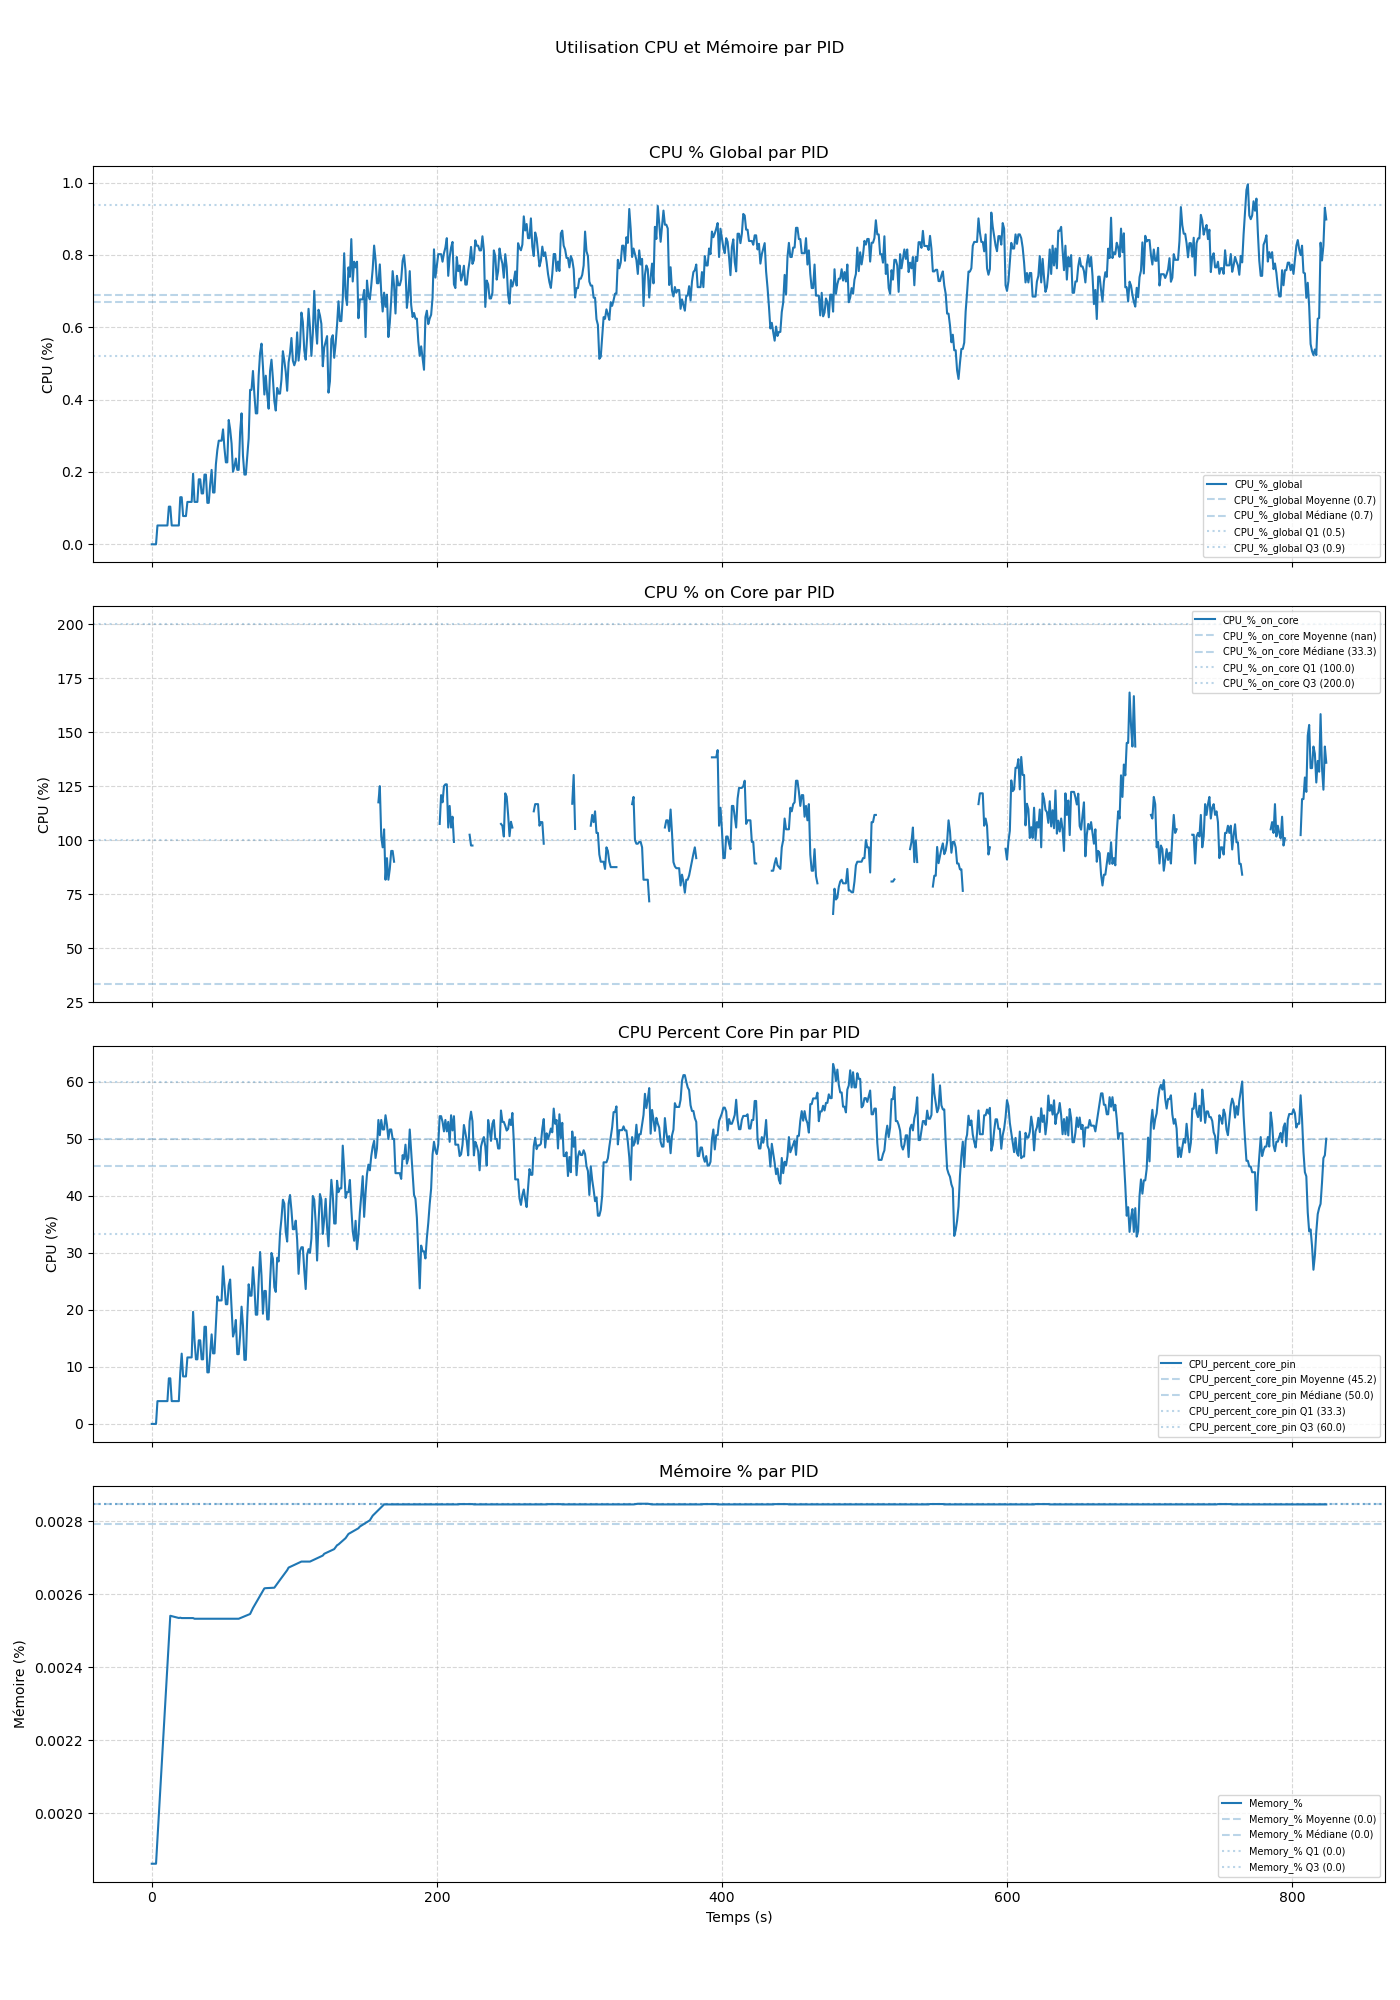
\includegraphics[width=\linewidth]{odb/cpu-conso-FE-16K.png}
                \centering\small Conso FE CPU/RAM ODB (16Ko)
            \end{column}

            \begin{column}{0.48\textwidth}
                
\includegraphics[width=\linewidth]{vanilla/cpu-conso-FE-16K.png}
                \centering\small Conso FE CPU/RAM Vanilla (16Ko)
            \end{column}
        
        \end{columns}
    \end{card}
\end{frame}

\begin{frame}{Consommation CPU et RAM, Payload 16Ko (IS)}
    \begin{card}
        \begin{columns}

            \begin{column}{0.48\textwidth}
                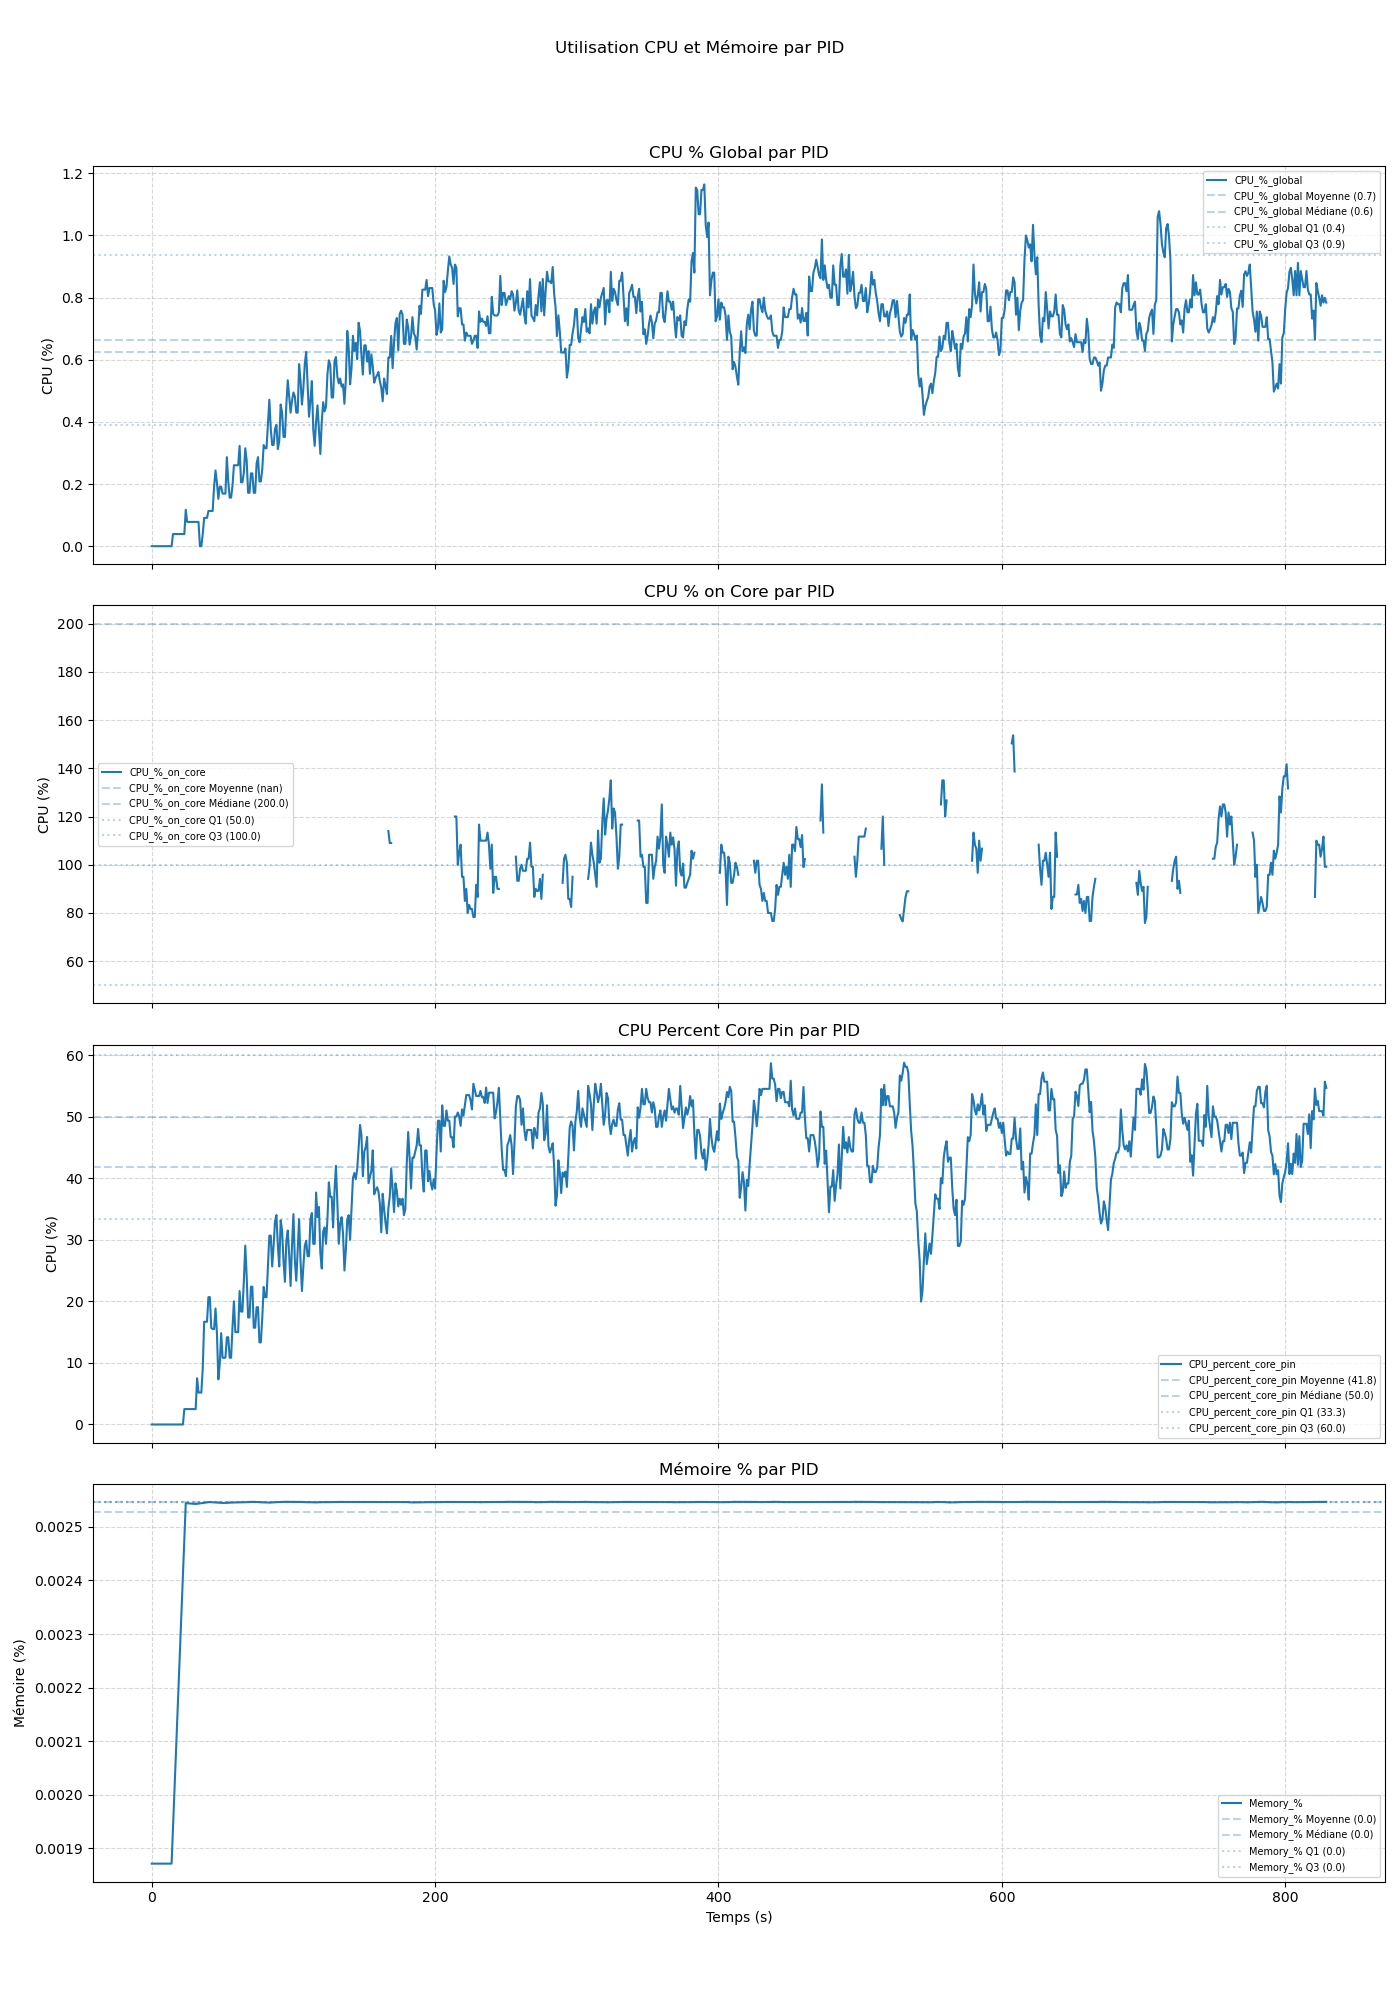
\includegraphics[width=\linewidth]{odb/cpu-conso-IS-16K.png}
                \centering\small Conso IS CPU/RAM ODB (16Ko)
            \end{column}

            \begin{column}{0.48\textwidth}
                
\includegraphics[width=\linewidth]{vanilla/cpu-conso-IS-16K.png}
                \centering\small Conso IS CPU/RAM Vanilla (16Ko)
            \end{column}
        
        \end{columns}
    \end{card}
\end{frame}

\begin{frame}{Consommation CPU et RAM, Payload 16Ko (BE)}
    \begin{card}
        \begin{columns}

            \begin{column}{0.48\textwidth}
                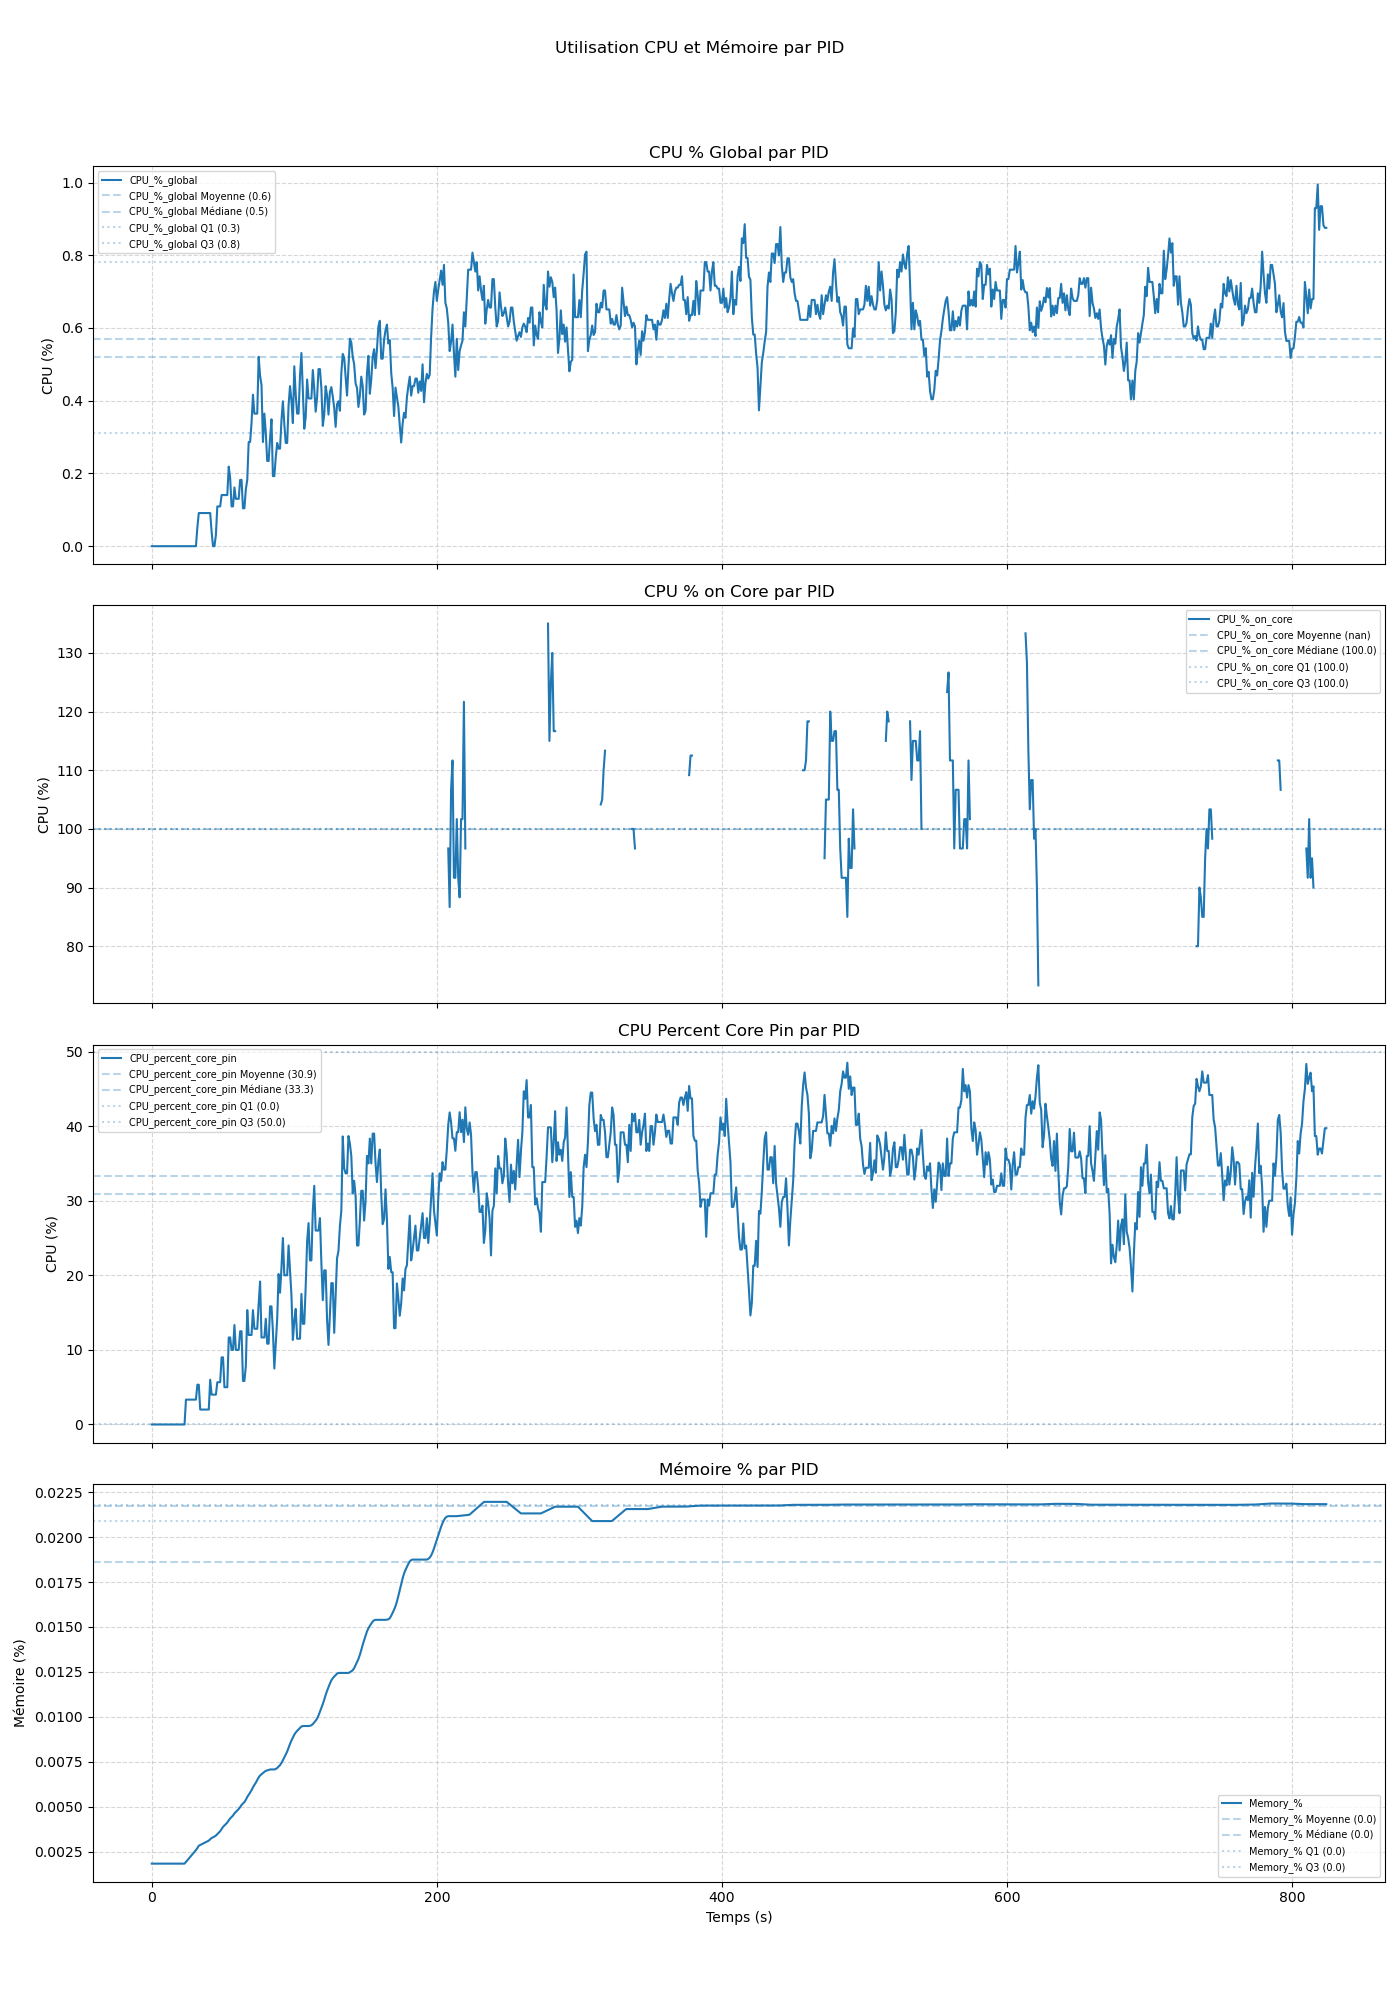
\includegraphics[width=\linewidth]{odb/cpu-conso-BE-16K.png}
                \centering\small Conso BE CPU/RAM ODB (16Ko)
            \end{column}

            \begin{column}{0.48\textwidth}
                
\includegraphics[width=\linewidth]{vanilla/cpu-conso-BE-16K.png}
                \centering\small Conso BE CPU/RAM Vanilla (16Ko)
            \end{column}
        
        \end{columns}
    \end{card}
\end{frame}

\begin{frame}{Temps de réponse moyen, Payload 16Ko}
    \begin{card}
        \begin{columns}

            \begin{column}{0.48\textwidth}
                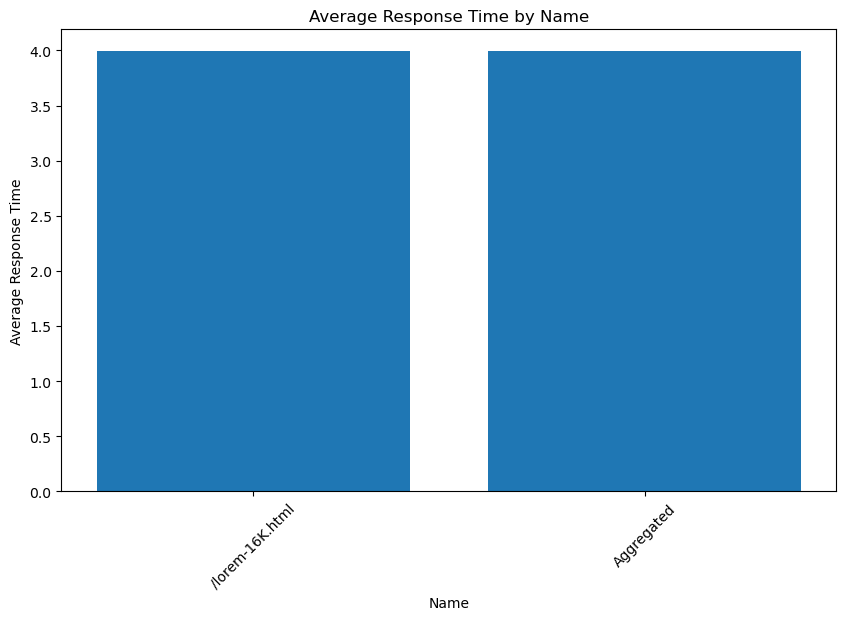
\includegraphics[width=\linewidth]{odb/avg-rtt-16K.png}
                \centering\small Temps de réponse moyen ODB (16Ko)
            \end{column}

            \begin{column}{0.48\textwidth}
                
\includegraphics[width=\linewidth]{vanilla/avg-rtt-16K.png}
                \centering\small Temps de réponse moyen Vanilla (16Ko)
            \end{column}
        
        \end{columns}
    \end{card}
\end{frame}


%%%%%%%%%%%%%%%%%%%%%%%%%%%%%%%%%%%%%%%%%%%%%%%%%
% Consommation CPU et RAM 32Ko
%%%%%%%%%%%%%%%%%%%%%%%%%%%%%%%%%%%%%%%%%%%%%%%%%
\begin{frame}{Consommation CPU et RAM, Payload 32Ko (FE)}
    \begin{card}
        \begin{columns}

            \begin{column}{0.48\textwidth}
                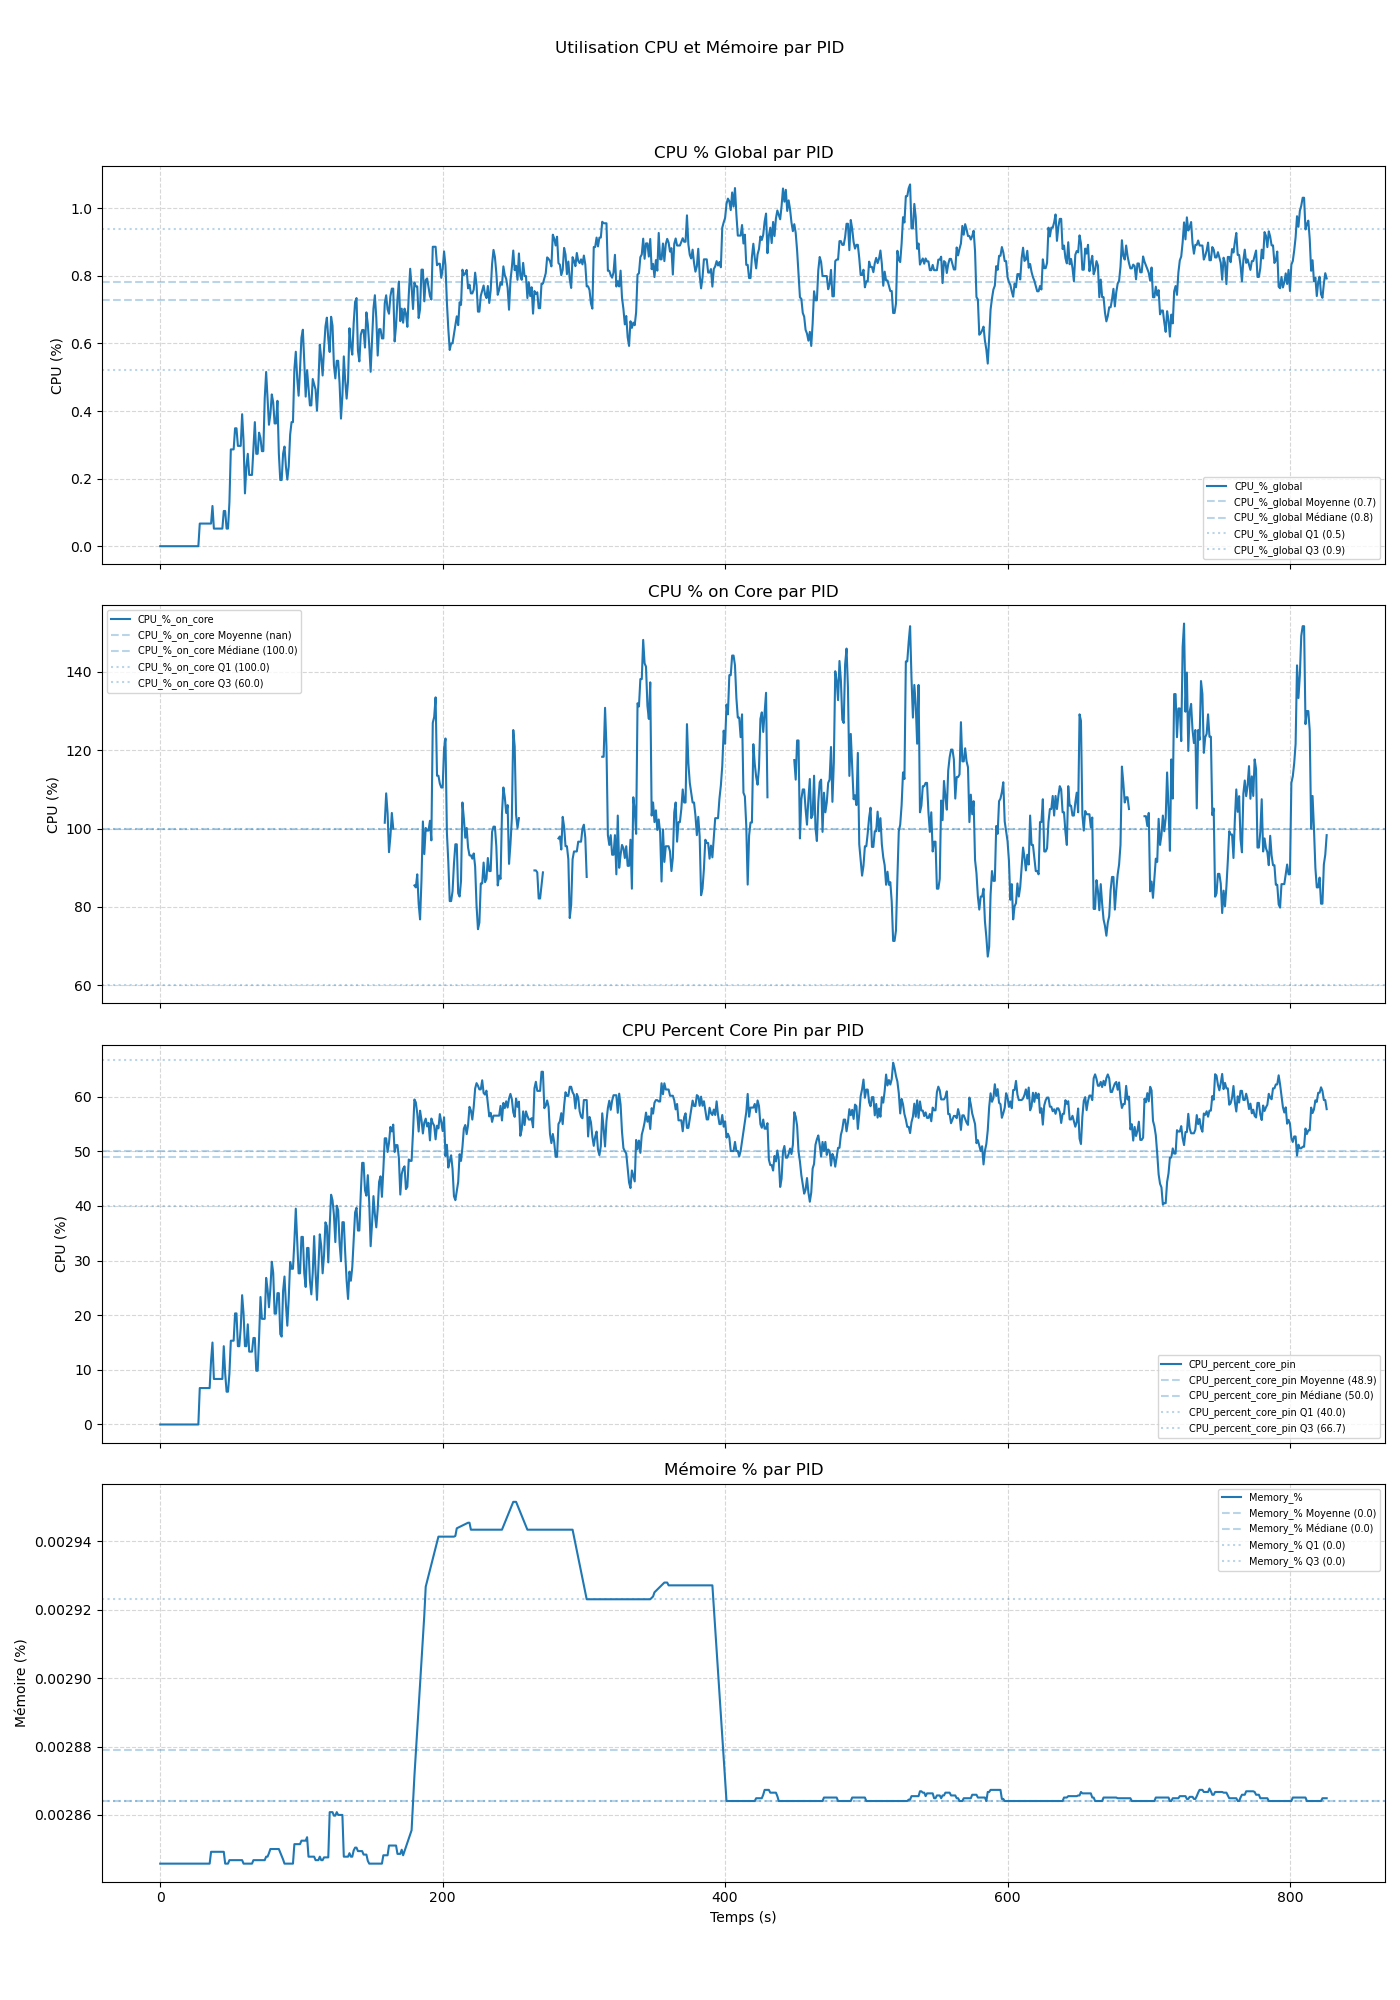
\includegraphics[width=\linewidth]{odb/cpu-conso-FE-32K.png}
                \centering\small Conso FE CPU/RAM ODB (32Ko)
            \end{column}

            \begin{column}{0.48\textwidth}
                
\includegraphics[width=\linewidth]{vanilla/cpu-conso-FE-32K.png}
                \centering\small Conso FE CPU/RAM Vanilla (32Ko)
            \end{column}
        
        \end{columns}
    \end{card}
\end{frame}

\begin{frame}{Consommation CPU et RAM, Payload 32Ko (IS)}
    \begin{card}
        \begin{columns}

            \begin{column}{0.48\textwidth}
                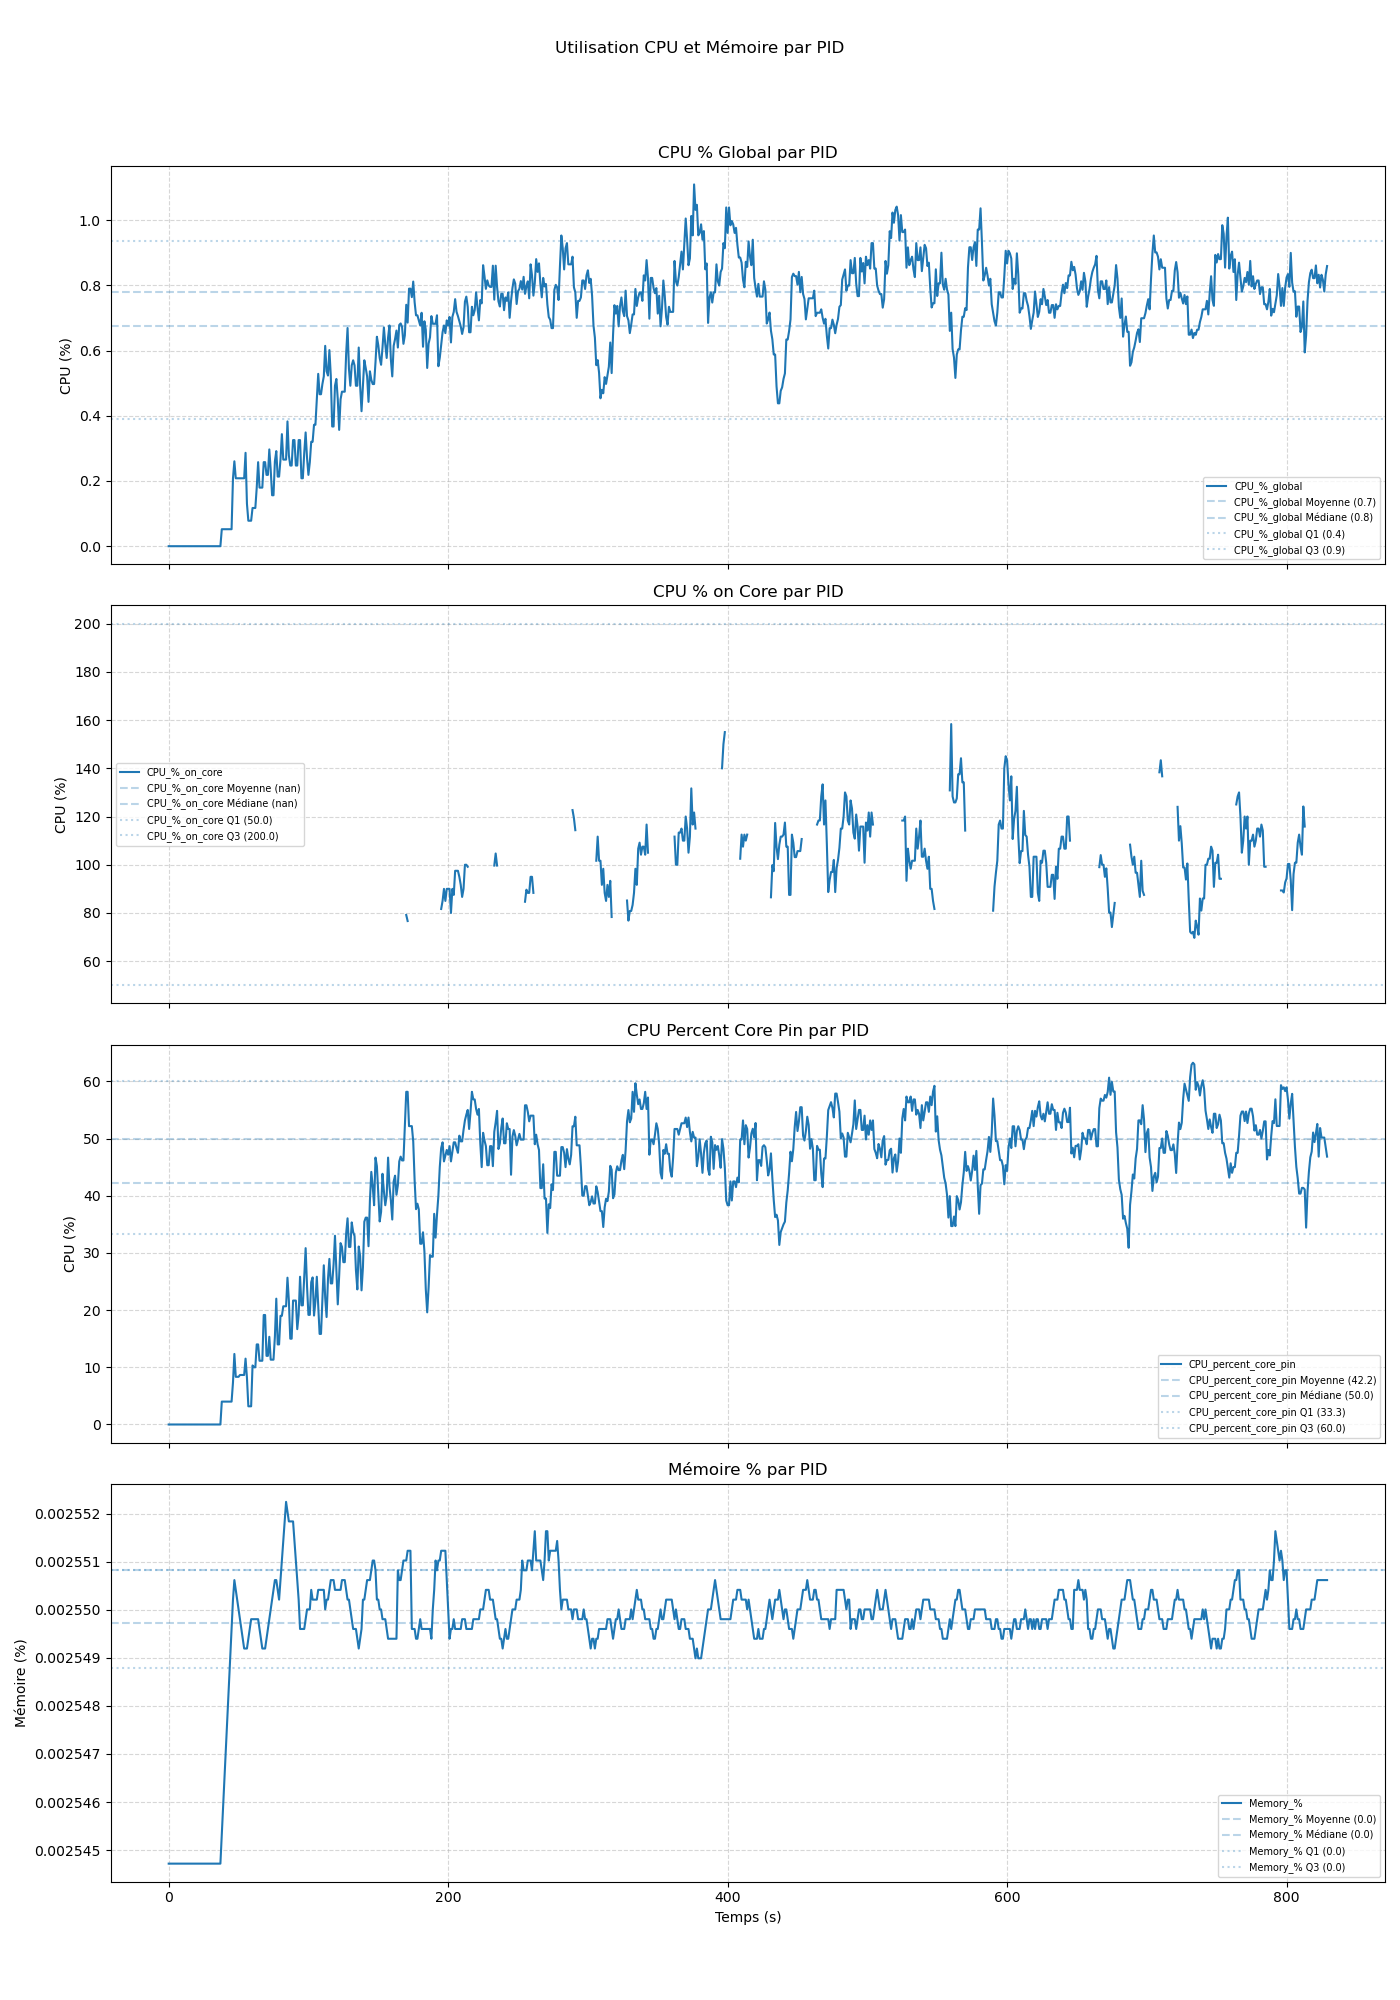
\includegraphics[width=\linewidth]{odb/cpu-conso-IS-32K.png}
                \centering\small Conso IS CPU/RAM ODB (32Ko)
            \end{column}

            \begin{column}{0.48\textwidth}
                
\includegraphics[width=\linewidth]{vanilla/cpu-conso-IS-32K.png}
                \centering\small Conso IS CPU/RAM Vanilla (32Ko)
            \end{column}
        
        \end{columns}
    \end{card}
\end{frame}

\begin{frame}{Consommation CPU et RAM, Payload 32Ko (BE)}
    \begin{card}
        \begin{columns}

            \begin{column}{0.48\textwidth}
                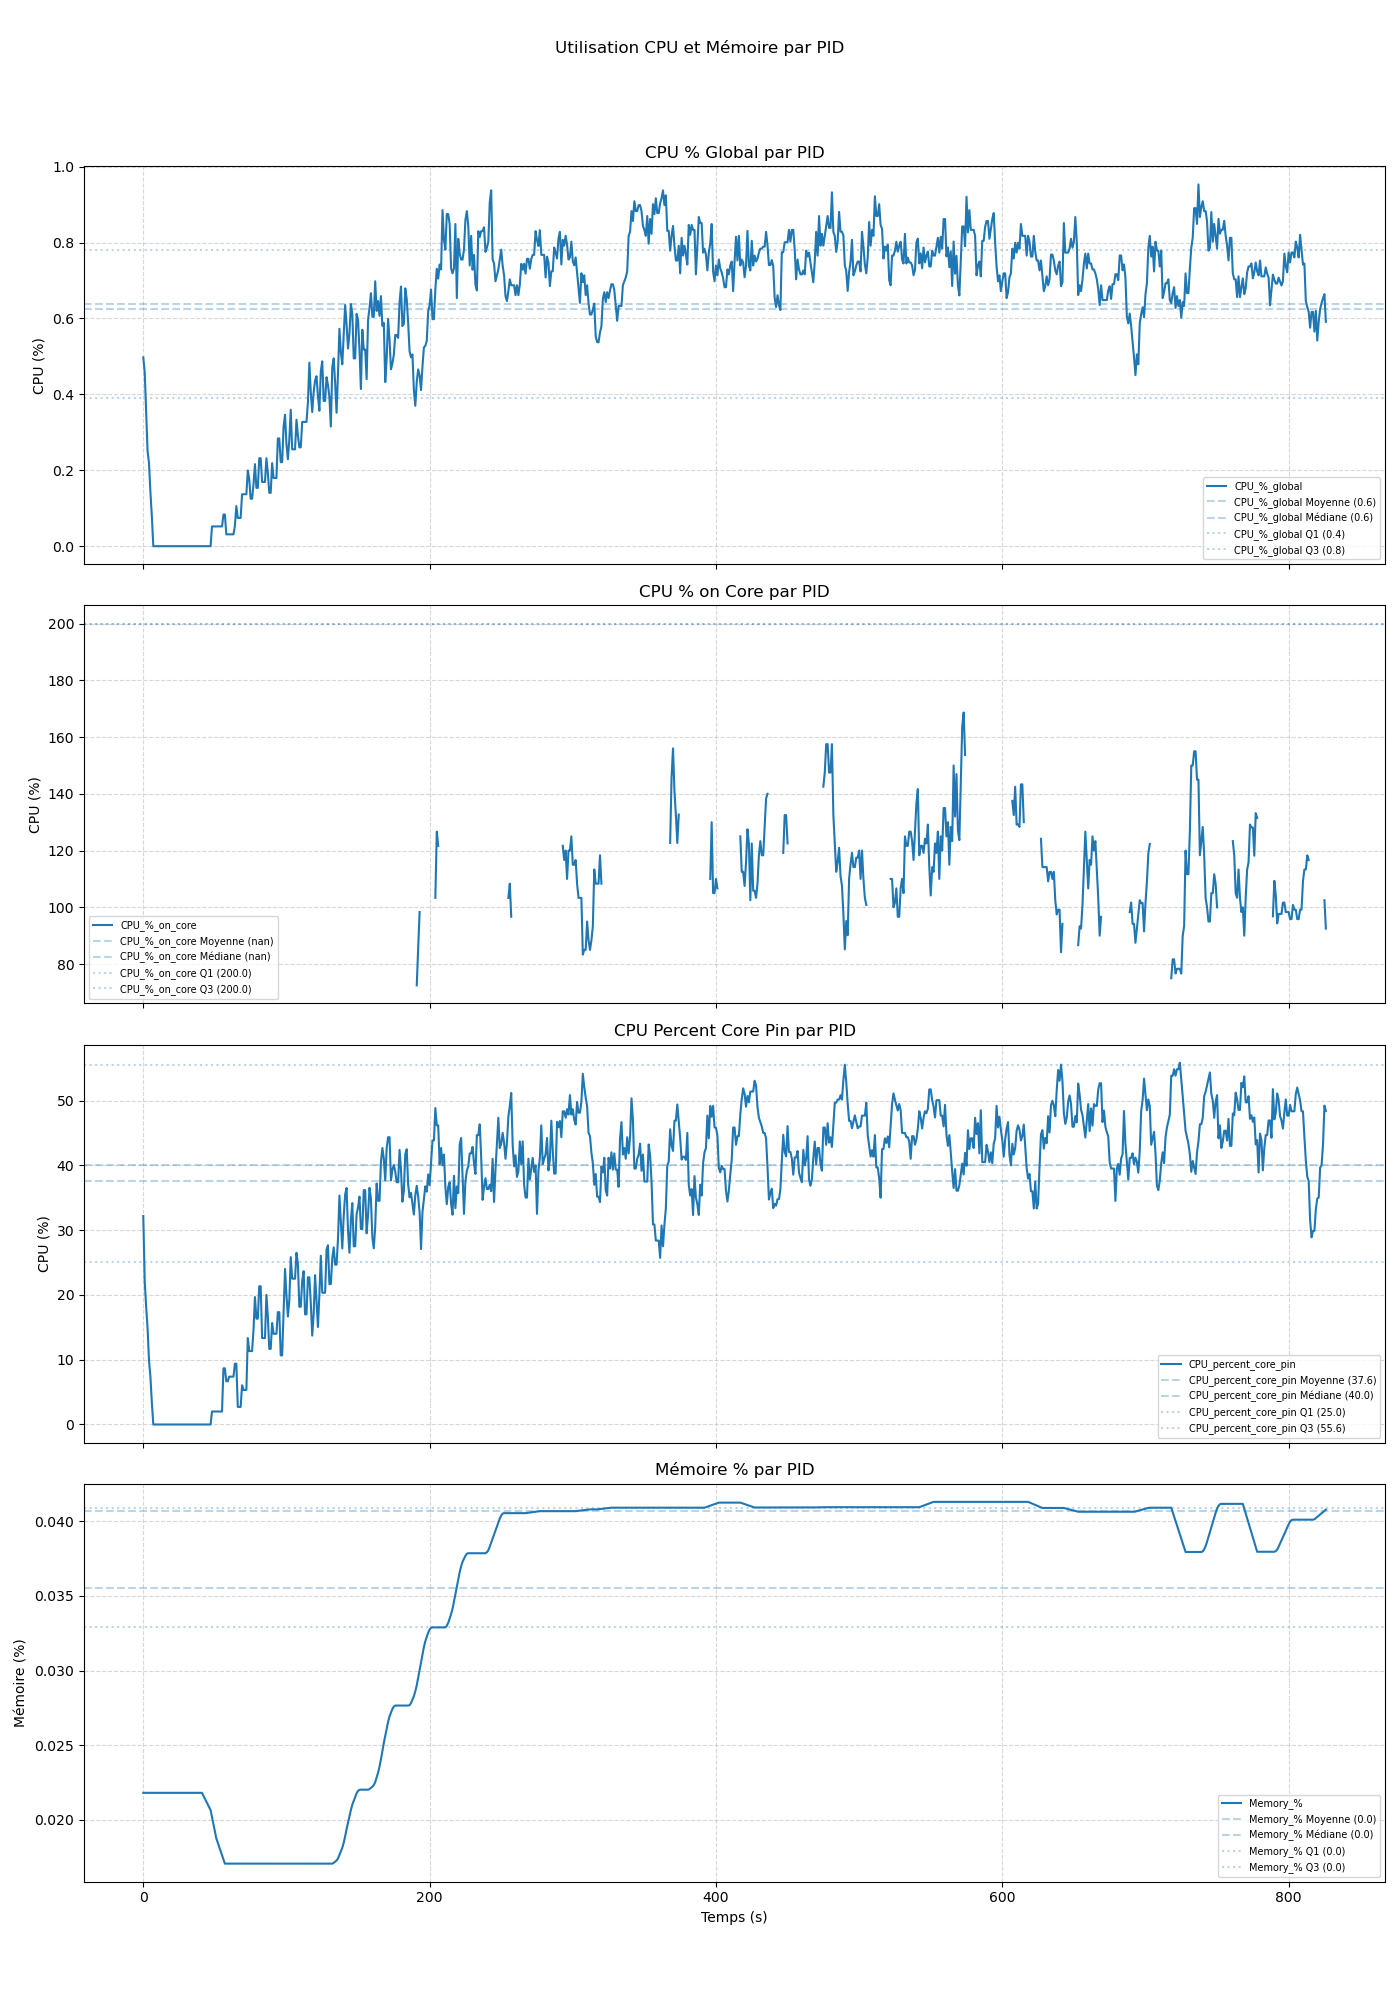
\includegraphics[width=\linewidth]{odb/cpu-conso-BE-32K.png}
                \centering\small Conso BE CPU/RAM ODB (32Ko)
            \end{column}

            \begin{column}{0.48\textwidth}
                
\includegraphics[width=\linewidth]{vanilla/cpu-conso-BE-32K.png}
                \centering\small Conso BE CPU/RAM Vanilla (32Ko)
            \end{column}
        
        \end{columns}
    \end{card}
\end{frame}

\begin{frame}{Temps de réponse moyen, Payload 32Ko}
    \begin{card}
        \begin{columns}

            \begin{column}{0.48\textwidth}
                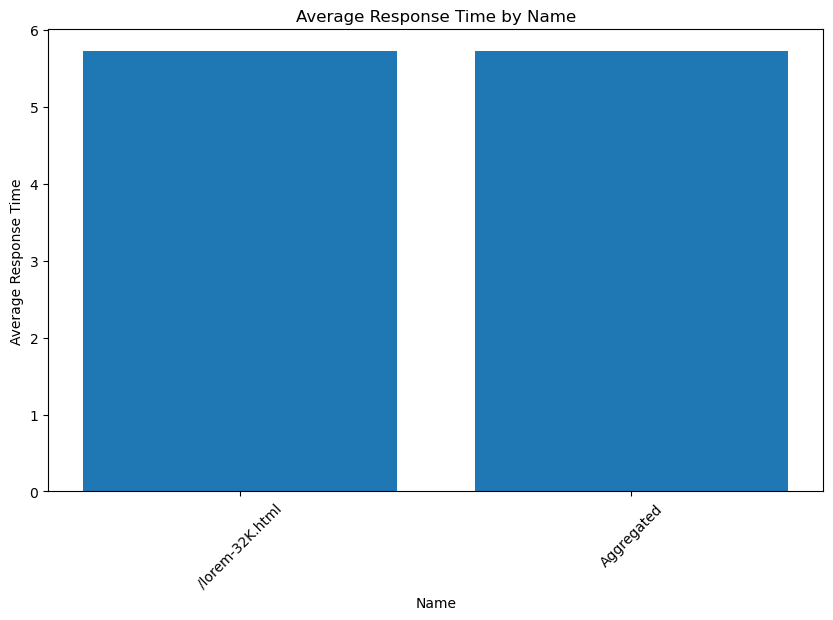
\includegraphics[width=\linewidth]{odb/avg-rtt-32K.png}
                \centering\small Temps de réponse moyen ODB (32Ko)
            \end{column}

            \begin{column}{0.48\textwidth}
                
\includegraphics[width=\linewidth]{vanilla/avg-rtt-32K.png}
                \centering\small Temps de réponse moyen Vanilla (32Ko)
            \end{column}
        
        \end{columns}
    \end{card}
\end{frame}

%%%%%%%%%%%%%%%%%%%%%%%%%%%%%%%%%%%%%%%%%%%%%%%%%
% Consommation CPU et RAM 64Ko
%%%%%%%%%%%%%%%%%%%%%%%%%%%%%%%%%%%%%%%%%%%%%%%%%
\begin{frame}{Consommation CPU et RAM, Payload 64Ko (FE)}
    \begin{card}
        \begin{columns}

            \begin{column}{0.48\textwidth}
                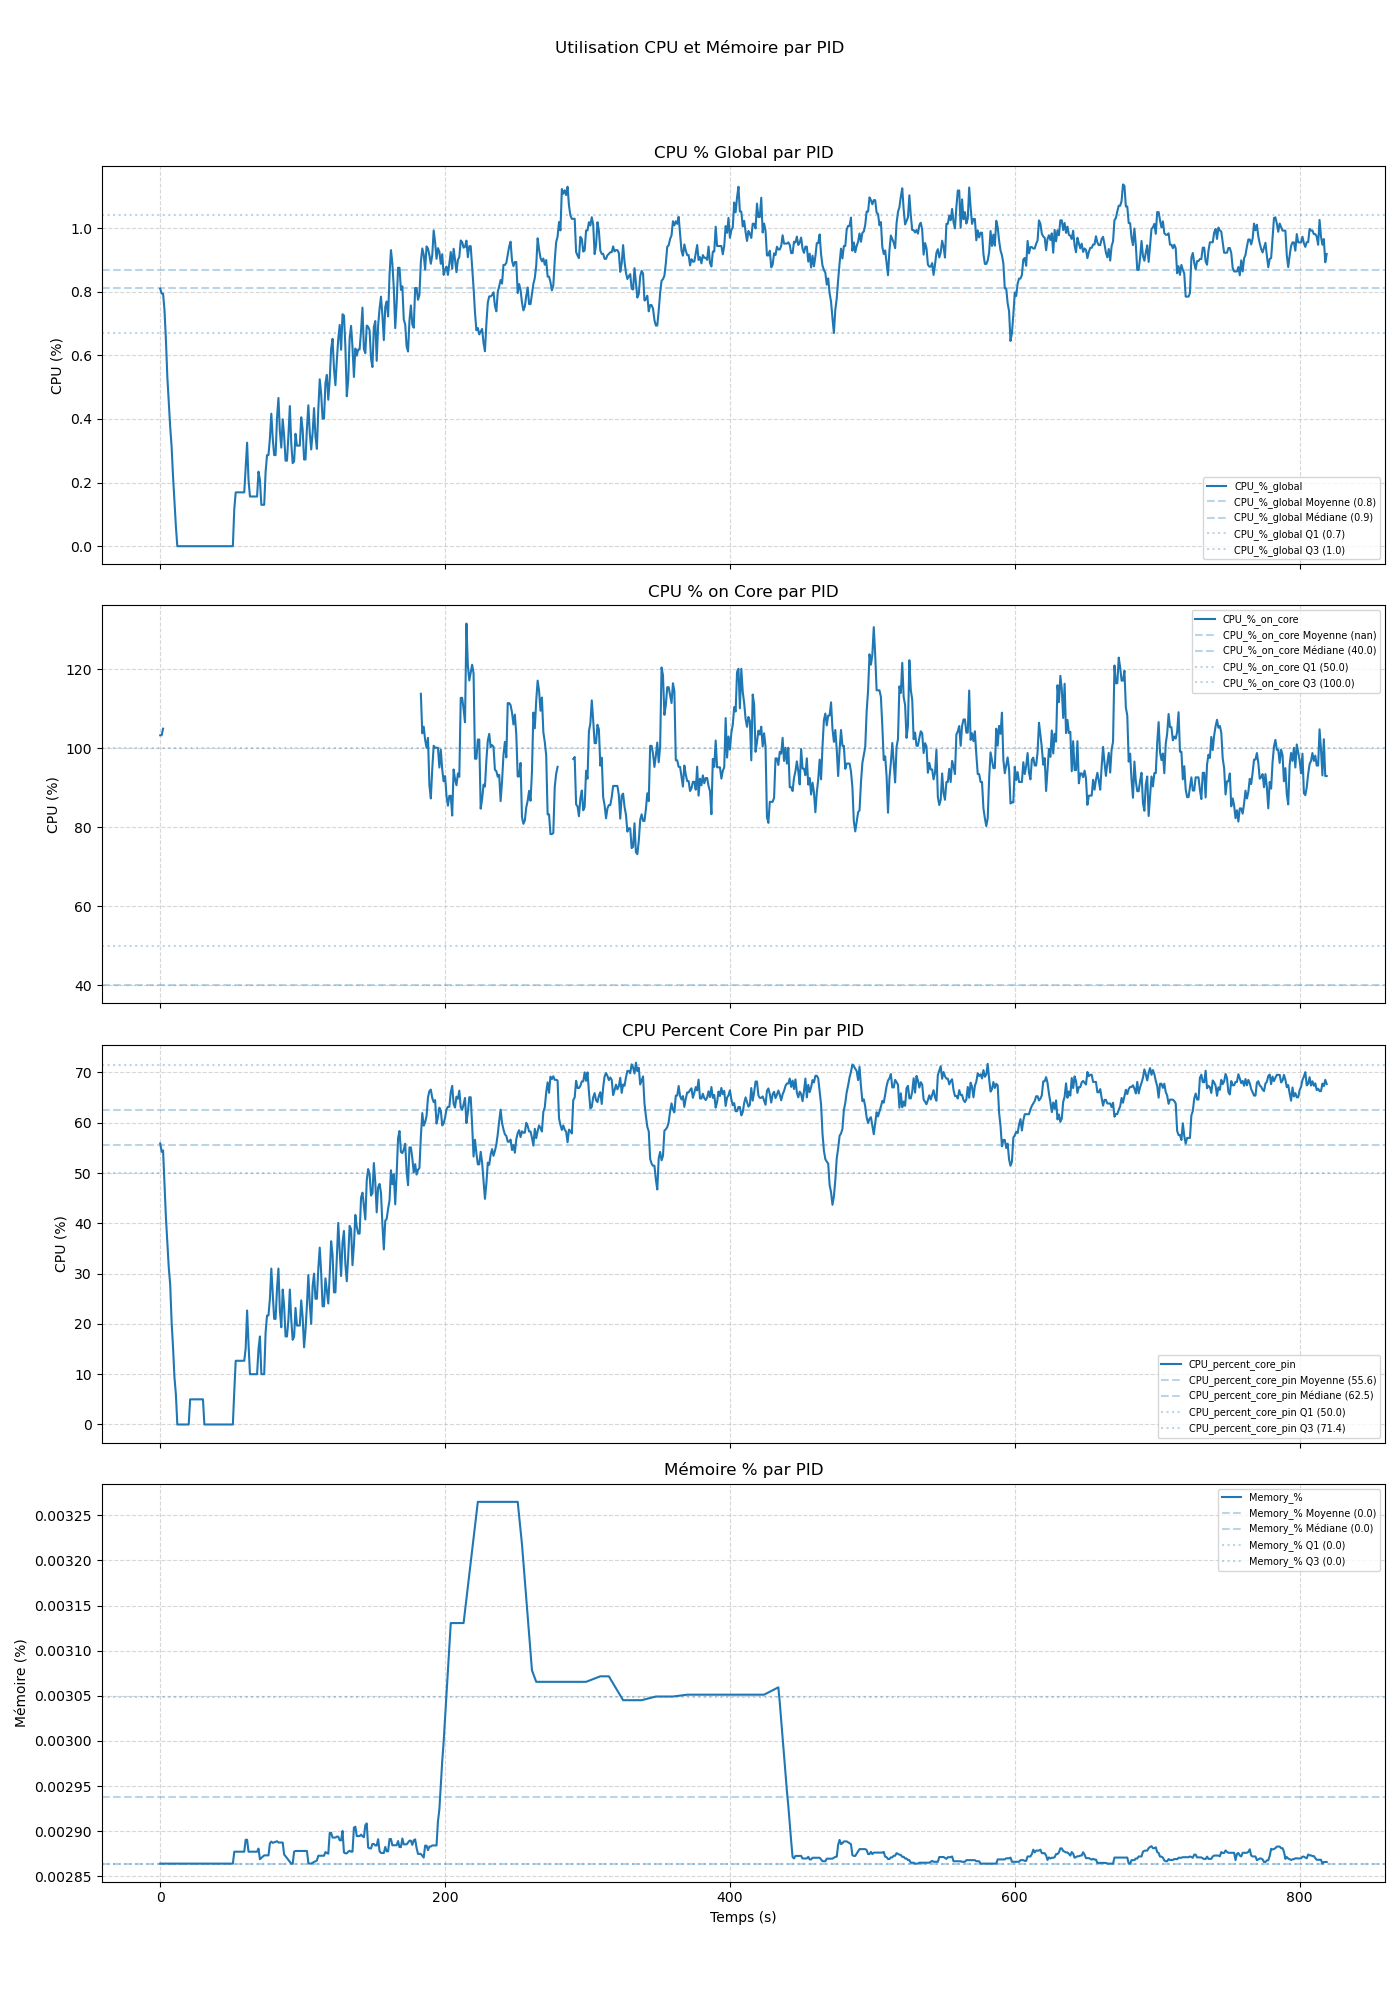
\includegraphics[width=\linewidth]{odb/cpu-conso-FE-64K.png}
                \centering\small Conso FE CPU/RAM ODB (64Ko)
            \end{column}

            \begin{column}{0.48\textwidth}
                
\includegraphics[width=\linewidth]{vanilla/cpu-conso-FE-64K.png}
                \centering\small Conso FE CPU/RAM Vanilla (64Ko)
            \end{column}
        
        \end{columns}
    \end{card}
\end{frame}

\begin{frame}{Consommation CPU et RAM, Payload 64Ko (IS)}
    \begin{card}
        \begin{columns}

            \begin{column}{0.48\textwidth}
                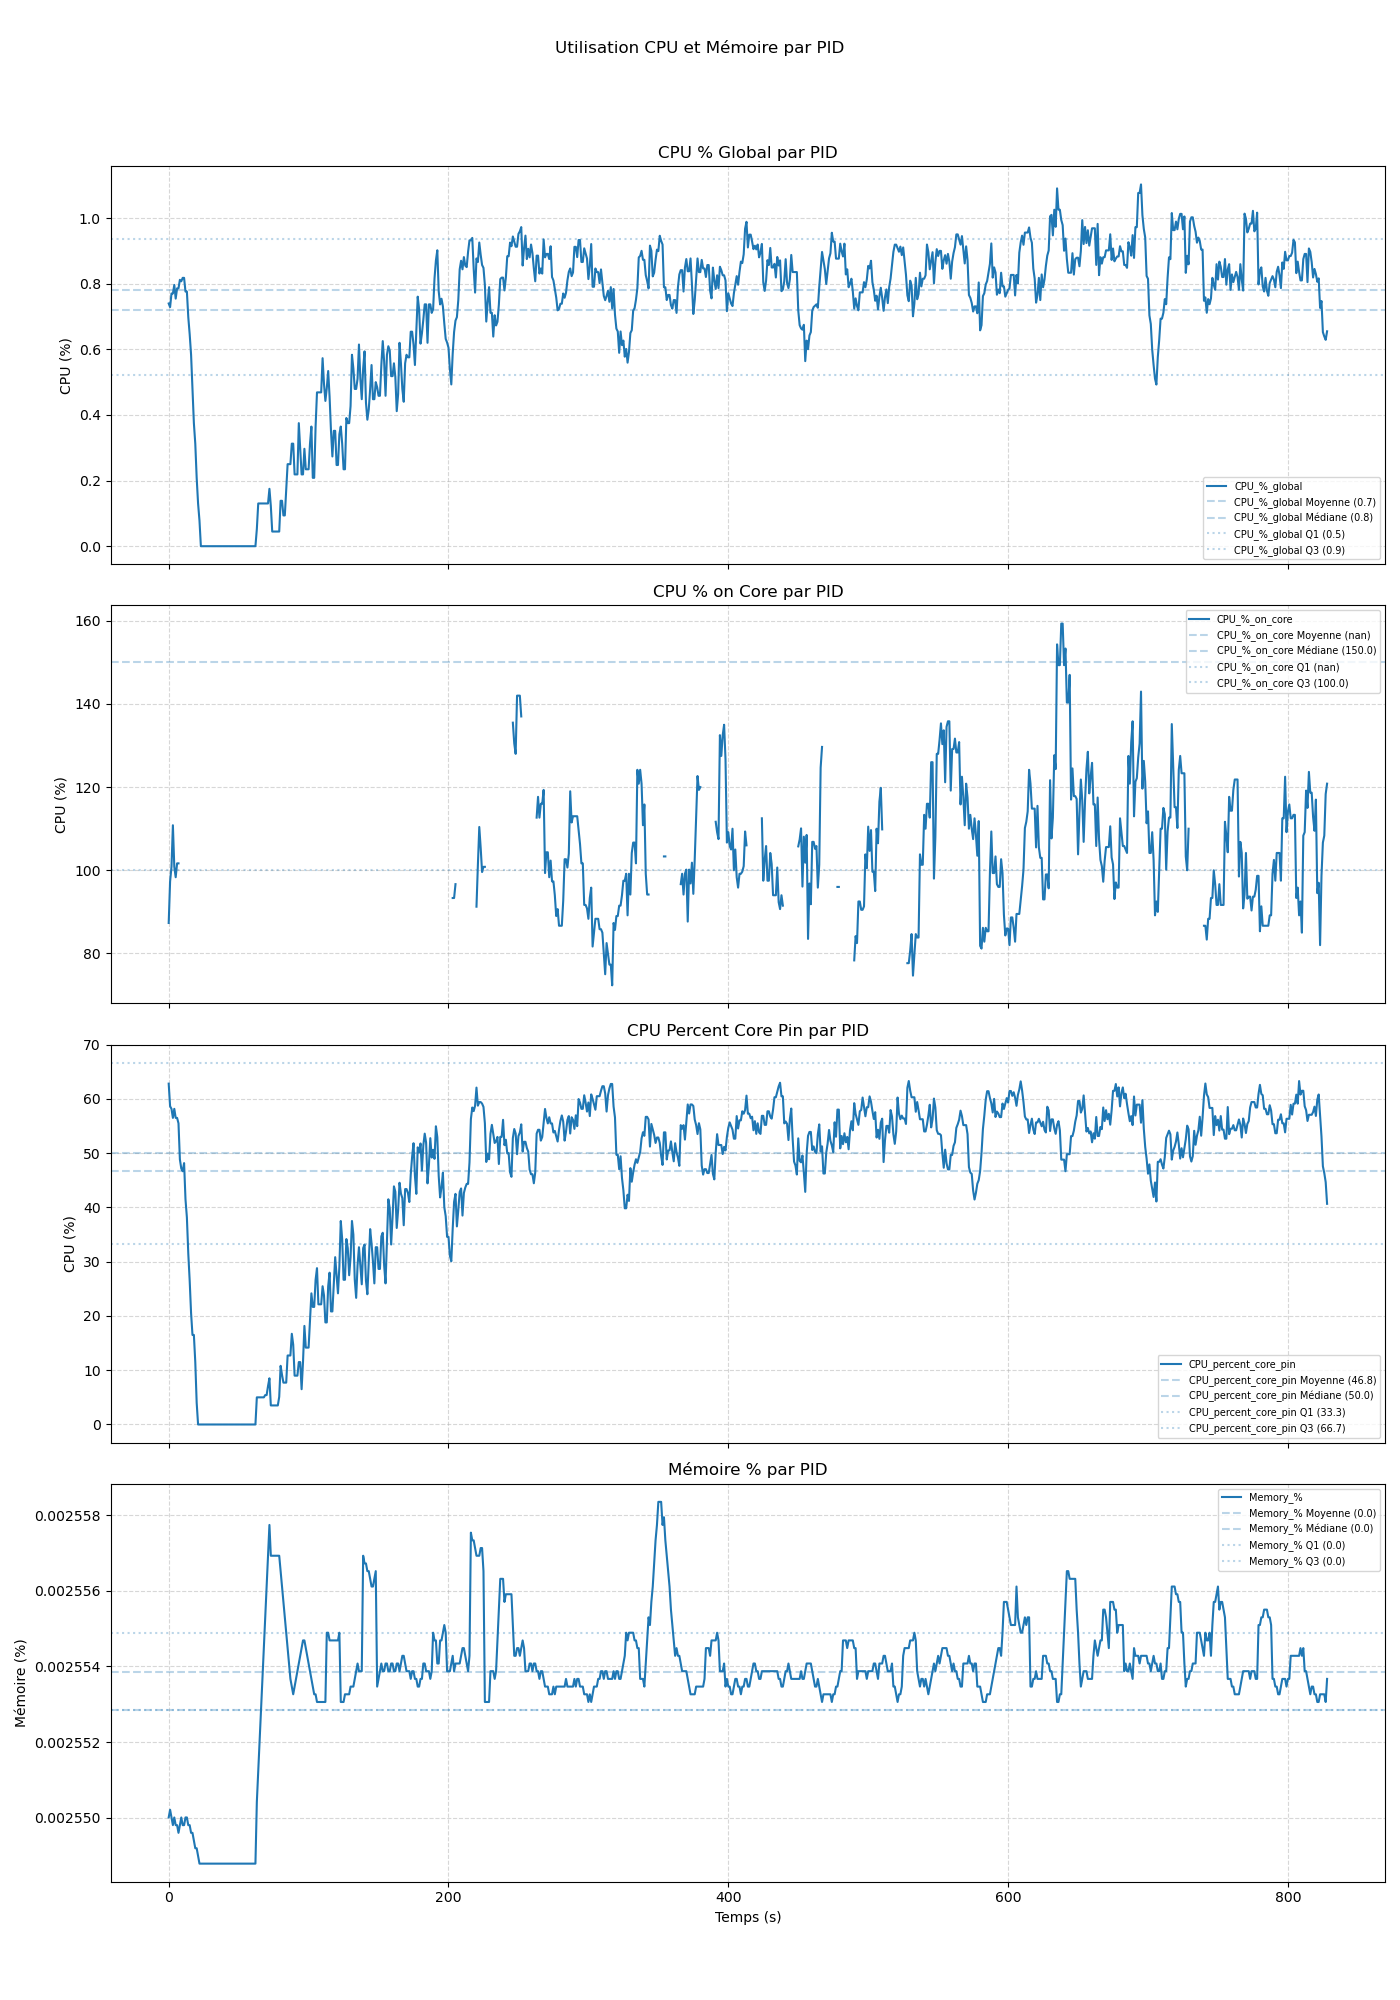
\includegraphics[width=\linewidth]{odb/cpu-conso-IS-64K.png}
                \centering\small Conso IS CPU/RAM ODB (64Ko)
            \end{column}

            \begin{column}{0.48\textwidth}
                
\includegraphics[width=\linewidth]{vanilla/cpu-conso-IS-64K.png}
                \centering\small Conso IS CPU/RAM Vanilla (64Ko)
            \end{column}
        
        \end{columns}
    \end{card}
\end{frame}

\begin{frame}{Consommation CPU et RAM, Payload 64Ko (BE)}
    \begin{card}
        \begin{columns}

            \begin{column}{0.48\textwidth}
                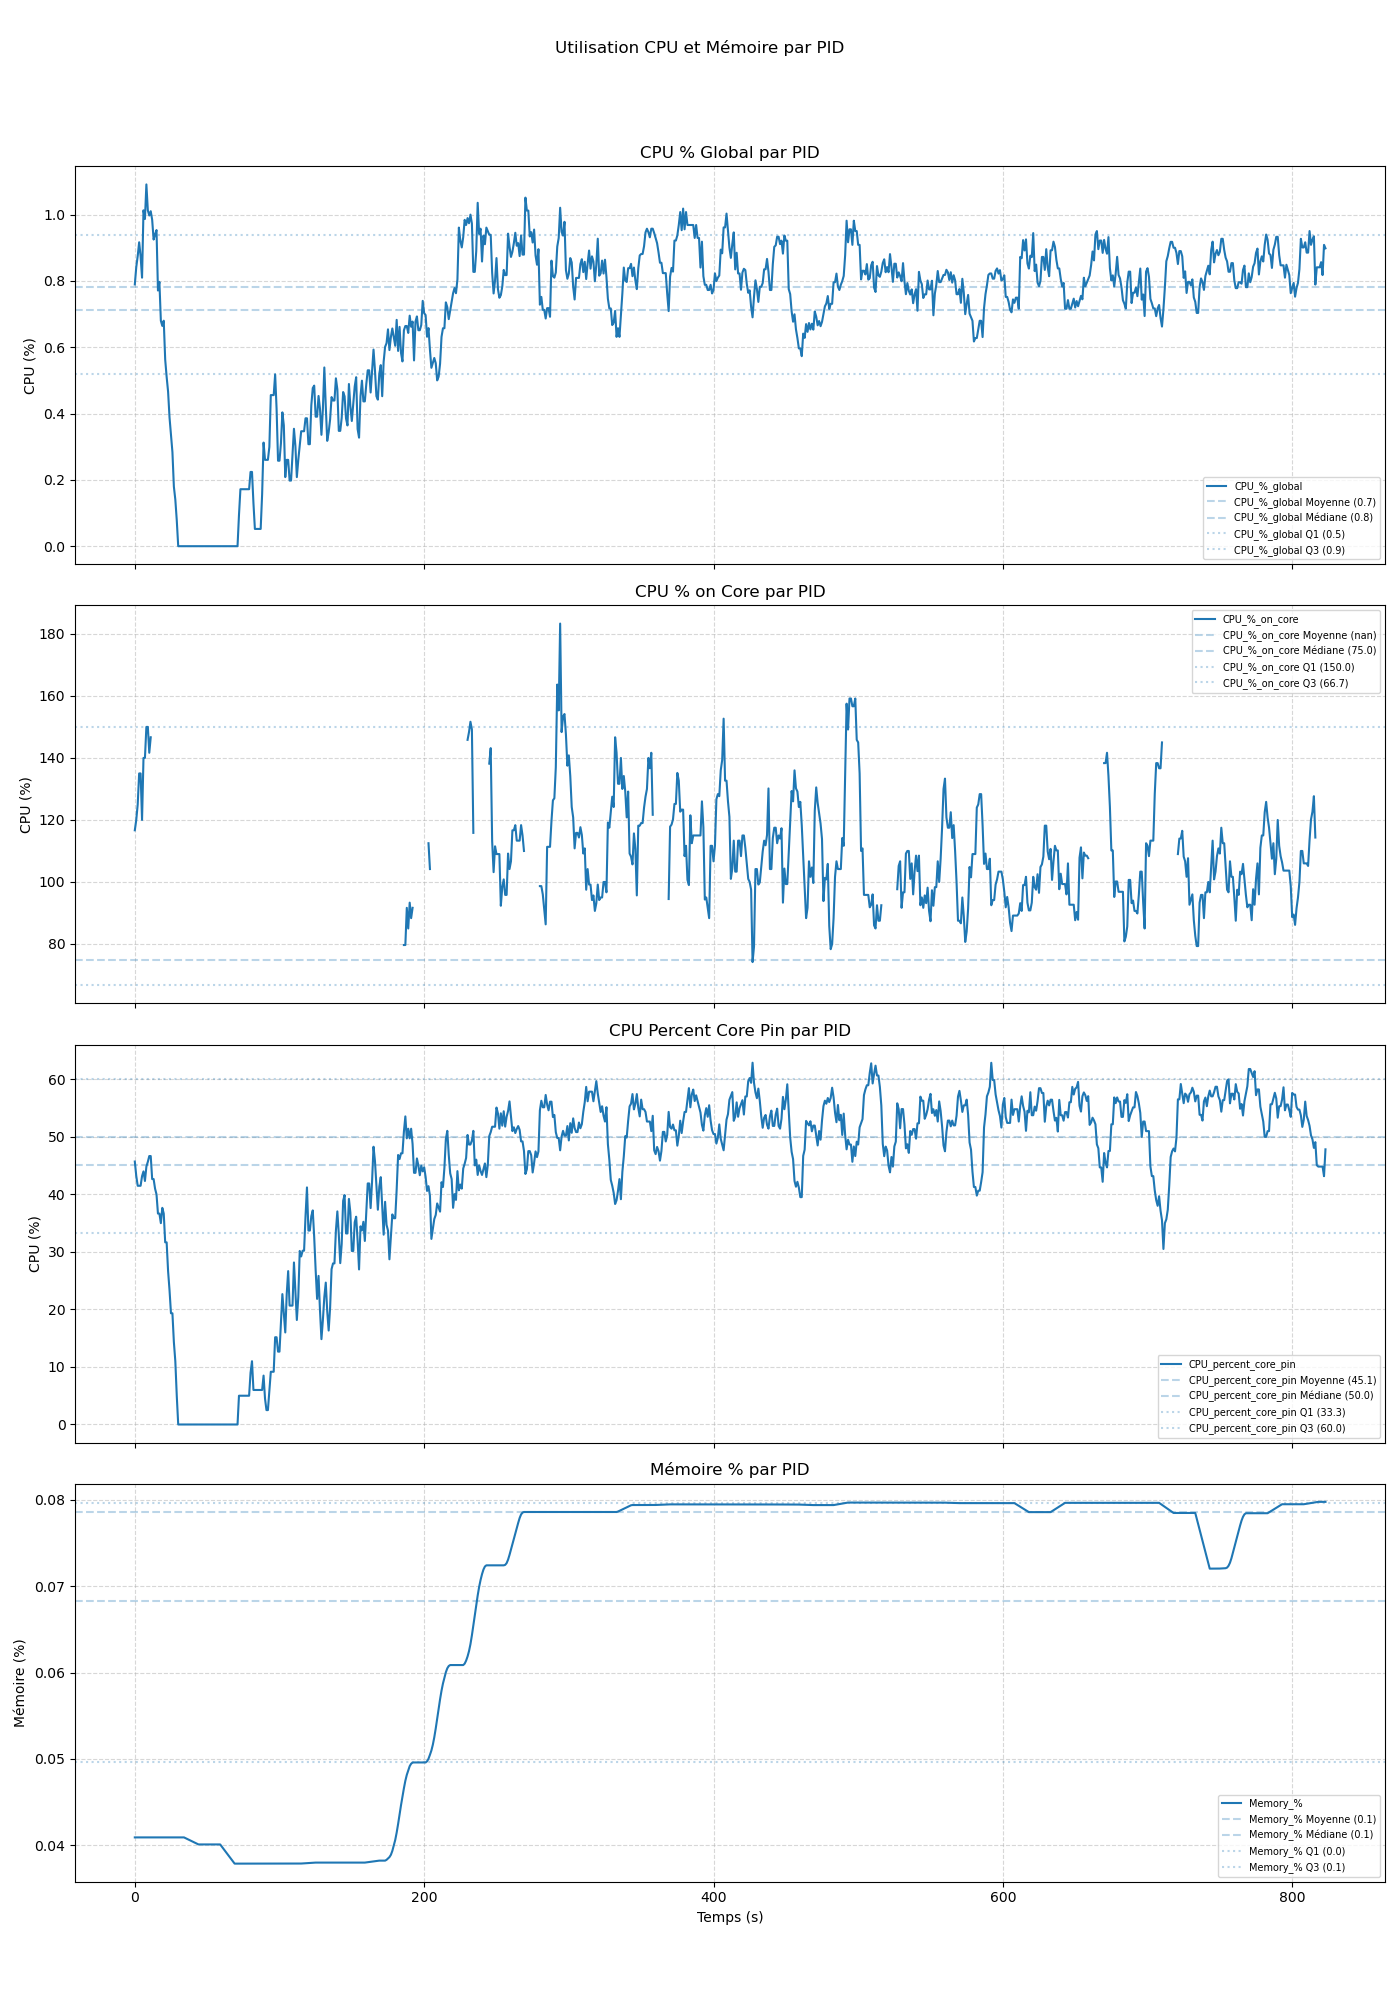
\includegraphics[width=\linewidth]{odb/cpu-conso-BE-64K.png}
                \centering\small Conso BE CPU/RAM ODB (64Ko)
            \end{column}

            \begin{column}{0.48\textwidth}
                
\includegraphics[width=\linewidth]{vanilla/cpu-conso-BE-64K.png}
                \centering\small Conso BE CPU/RAM Vanilla (64Ko)
            \end{column}
        
        \end{columns}
    \end{card}
\end{frame}

\begin{frame}{Temps de réponse moyen, Payload 64Ko}
    \begin{card}
        \begin{columns}

            \begin{column}{0.48\textwidth}
                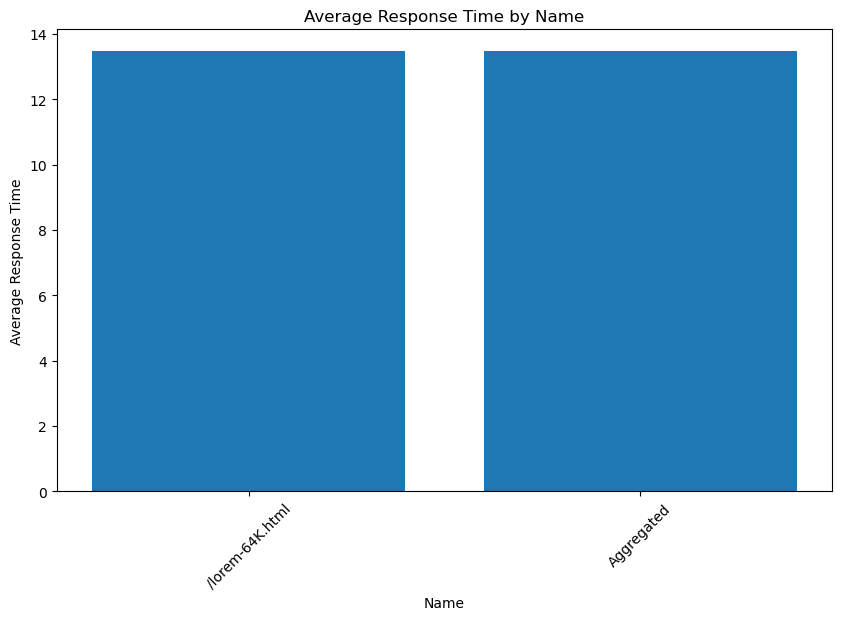
\includegraphics[width=\linewidth]{odb/avg-rtt-64K.png}
                \centering\small Temps de réponse moyen ODB (64Ko)
            \end{column}

            \begin{column}{0.48\textwidth}
                
\includegraphics[width=\linewidth]{vanilla/avg-rtt-64K.png}
                \centering\small Temps de réponse moyen Vanilla (64Ko)
            \end{column}
        
        \end{columns}
    \end{card}
\end{frame}


%%%%%%%%%%%%%%%%%%%%%%%%%%%%%%%%%%%%%%%%%%%%%%%%%
% Consommation CPU et RAM 128Ko
%%%%%%%%%%%%%%%%%%%%%%%%%%%%%%%%%%%%%%%%%%%%%%%%%
\begin{frame}{Consommation CPU et RAM, Payload 128Ko (FE)}
    \begin{card}
        \begin{columns}

            \begin{column}{0.48\textwidth}
                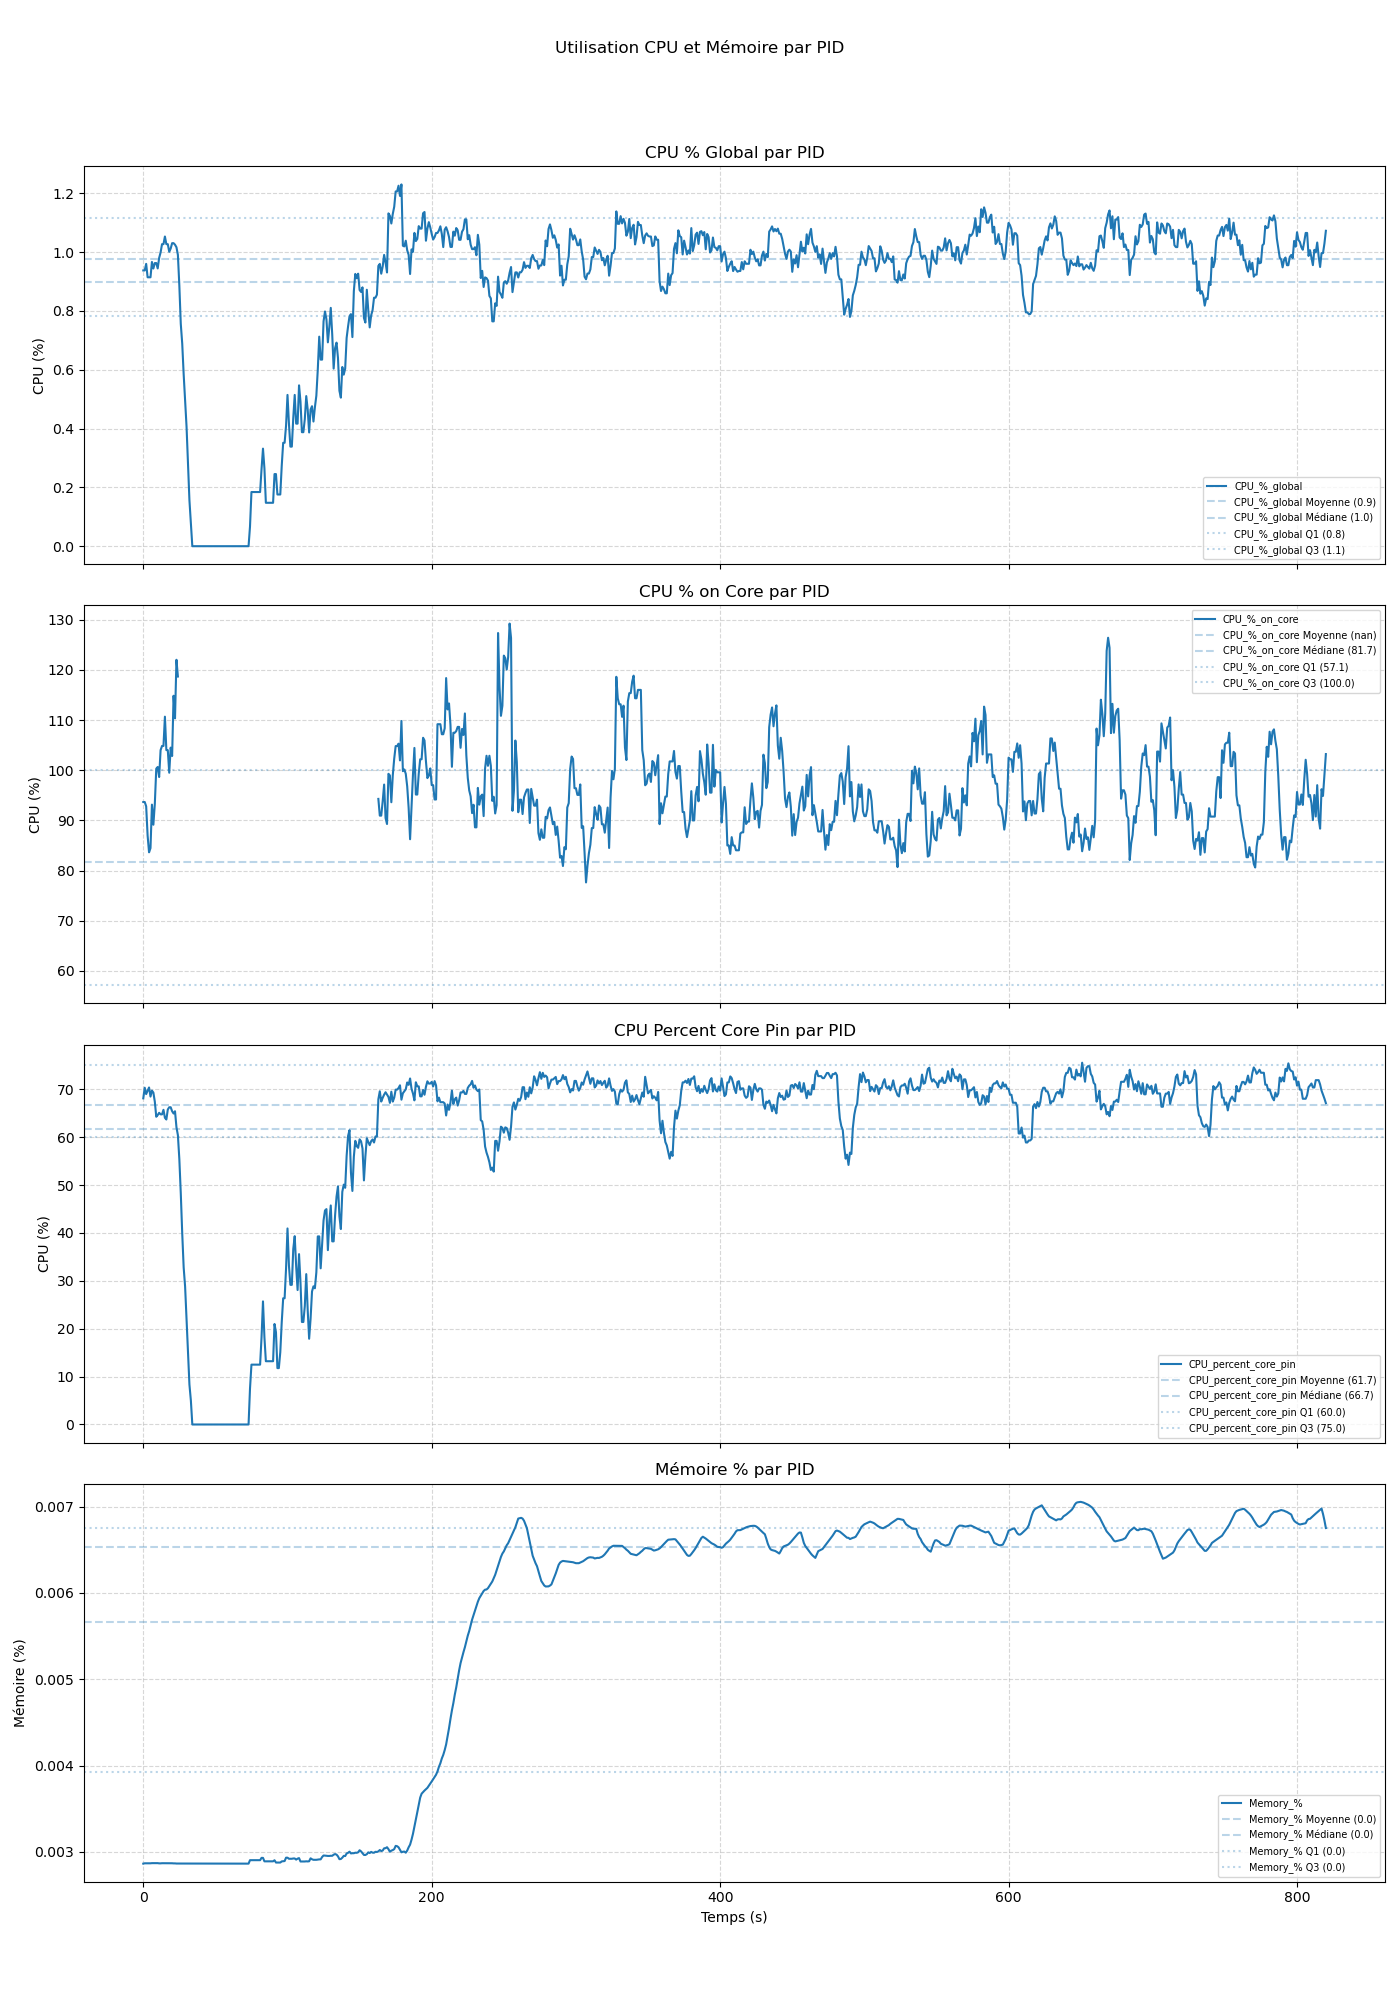
\includegraphics[width=\linewidth]{odb/cpu-conso-FE-128K.png}
                \centering\small Conso FE CPU/RAM ODB (128Ko)
            \end{column}

            \begin{column}{0.48\textwidth}
                
\includegraphics[width=\linewidth]{vanilla/cpu-conso-FE-128K.png}
                \centering\small Conso FE CPU/RAM Vanilla (128Ko)
            \end{column}
        
        \end{columns}
    \end{card}
\end{frame}

\begin{frame}{Consommation CPU et RAM, Payload 128Ko (IS)}
    \begin{card}
        \begin{columns}

            \begin{column}{0.48\textwidth}
                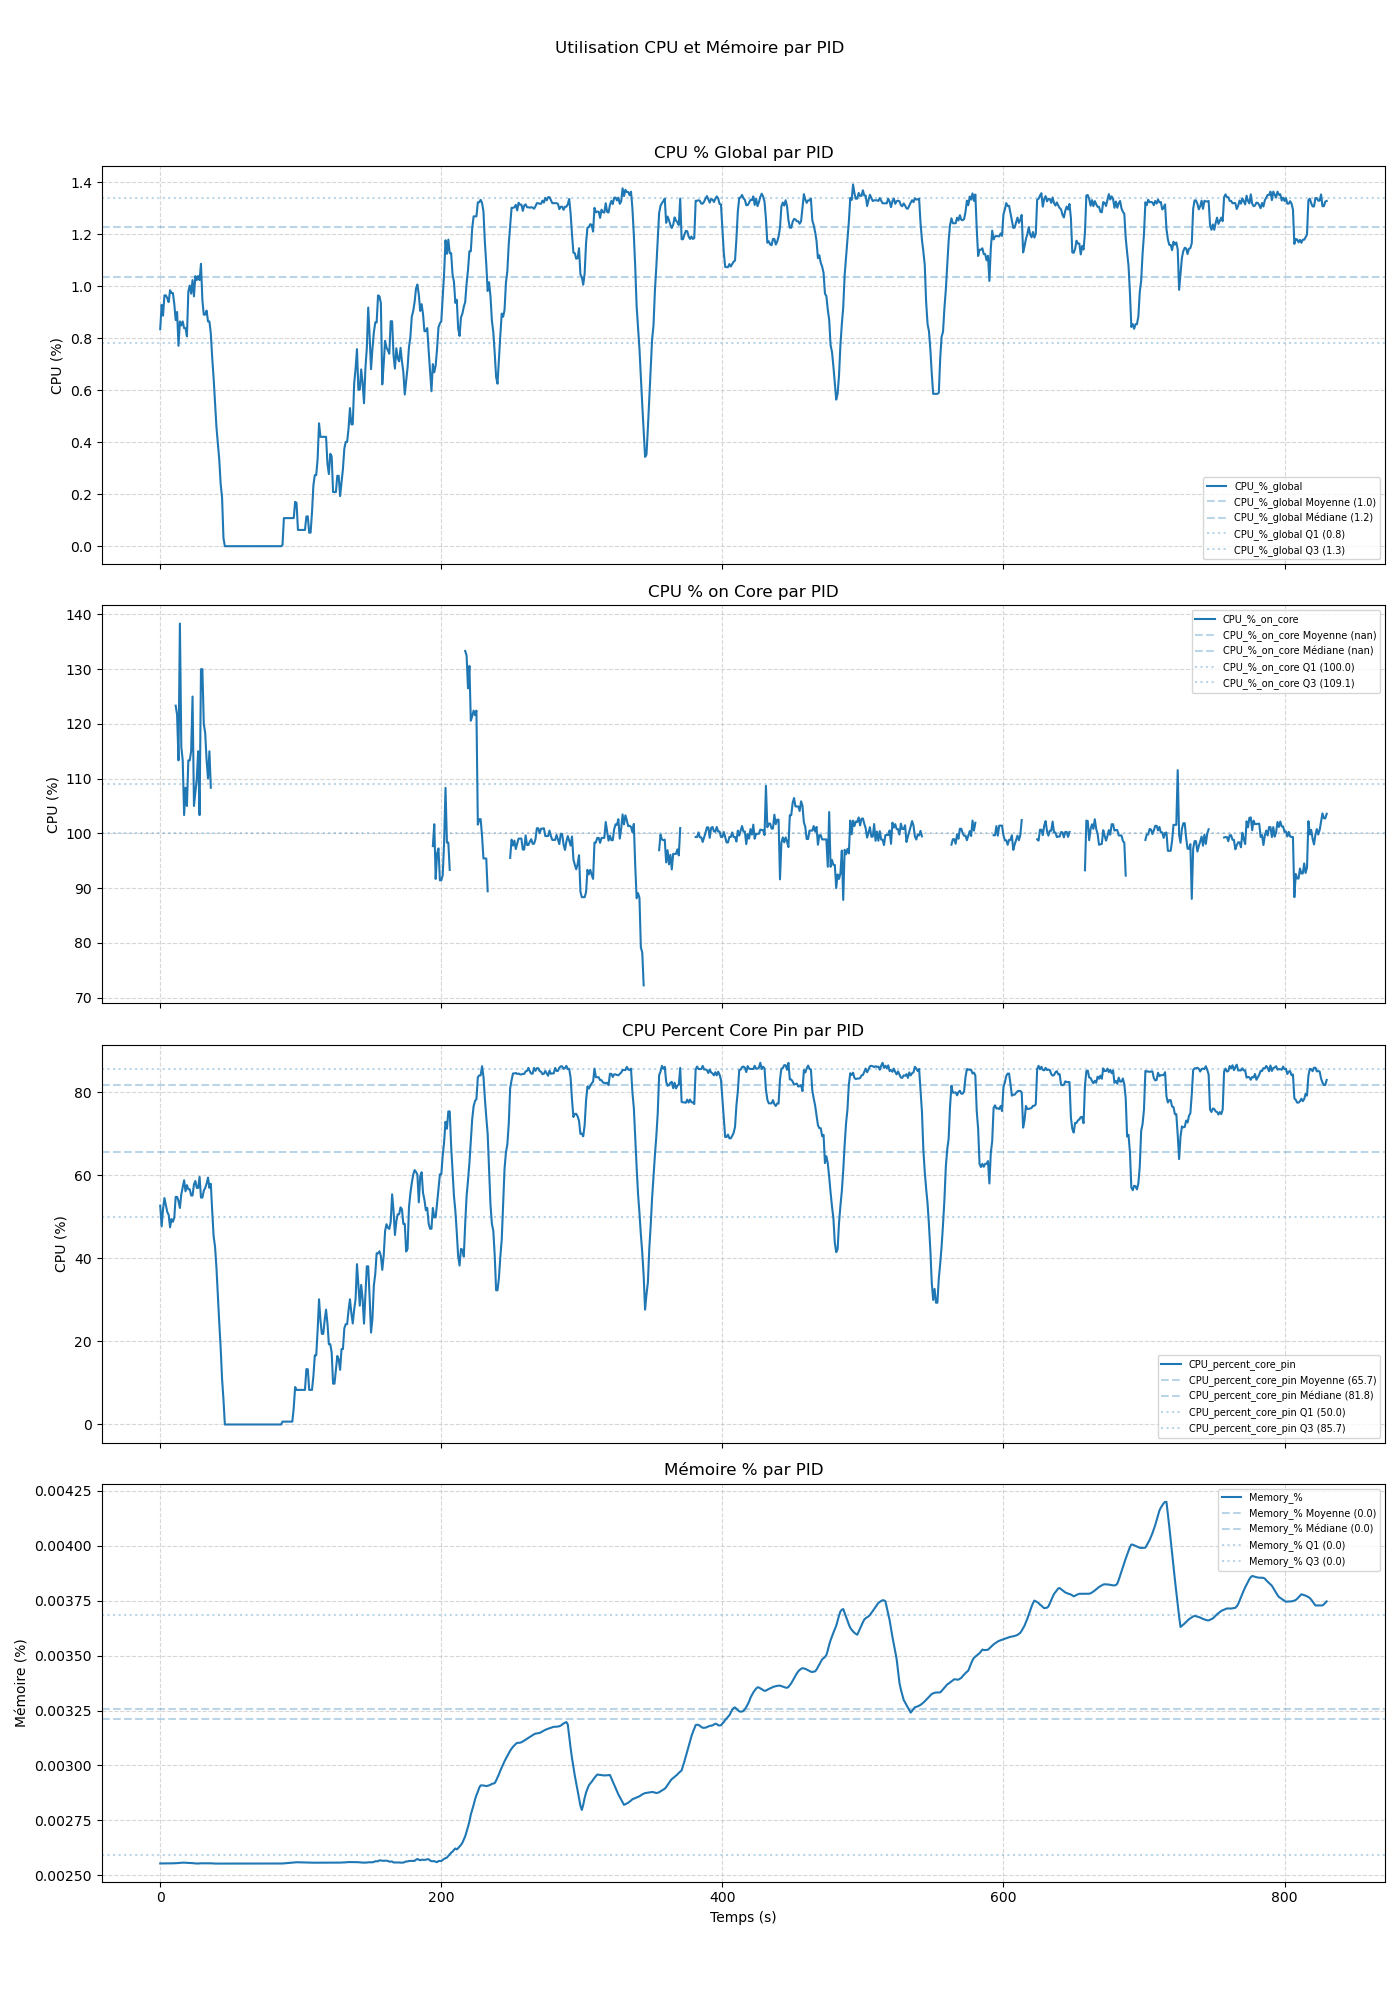
\includegraphics[width=\linewidth]{odb/cpu-conso-IS-128K.png}
                \centering\small Conso IS CPU/RAM ODB (128Ko)
            \end{column}

            \begin{column}{0.48\textwidth}
                
\includegraphics[width=\linewidth]{vanilla/cpu-conso-IS-128K.png}
                \centering\small Conso IS CPU/RAM Vanilla (128Ko)
            \end{column}
        
        \end{columns}
    \end{card}
\end{frame}

\begin{frame}{Consommation CPU et RAM, Payload 128Ko (BE)}
    \begin{card}
        \begin{columns}

            \begin{column}{0.48\textwidth}
                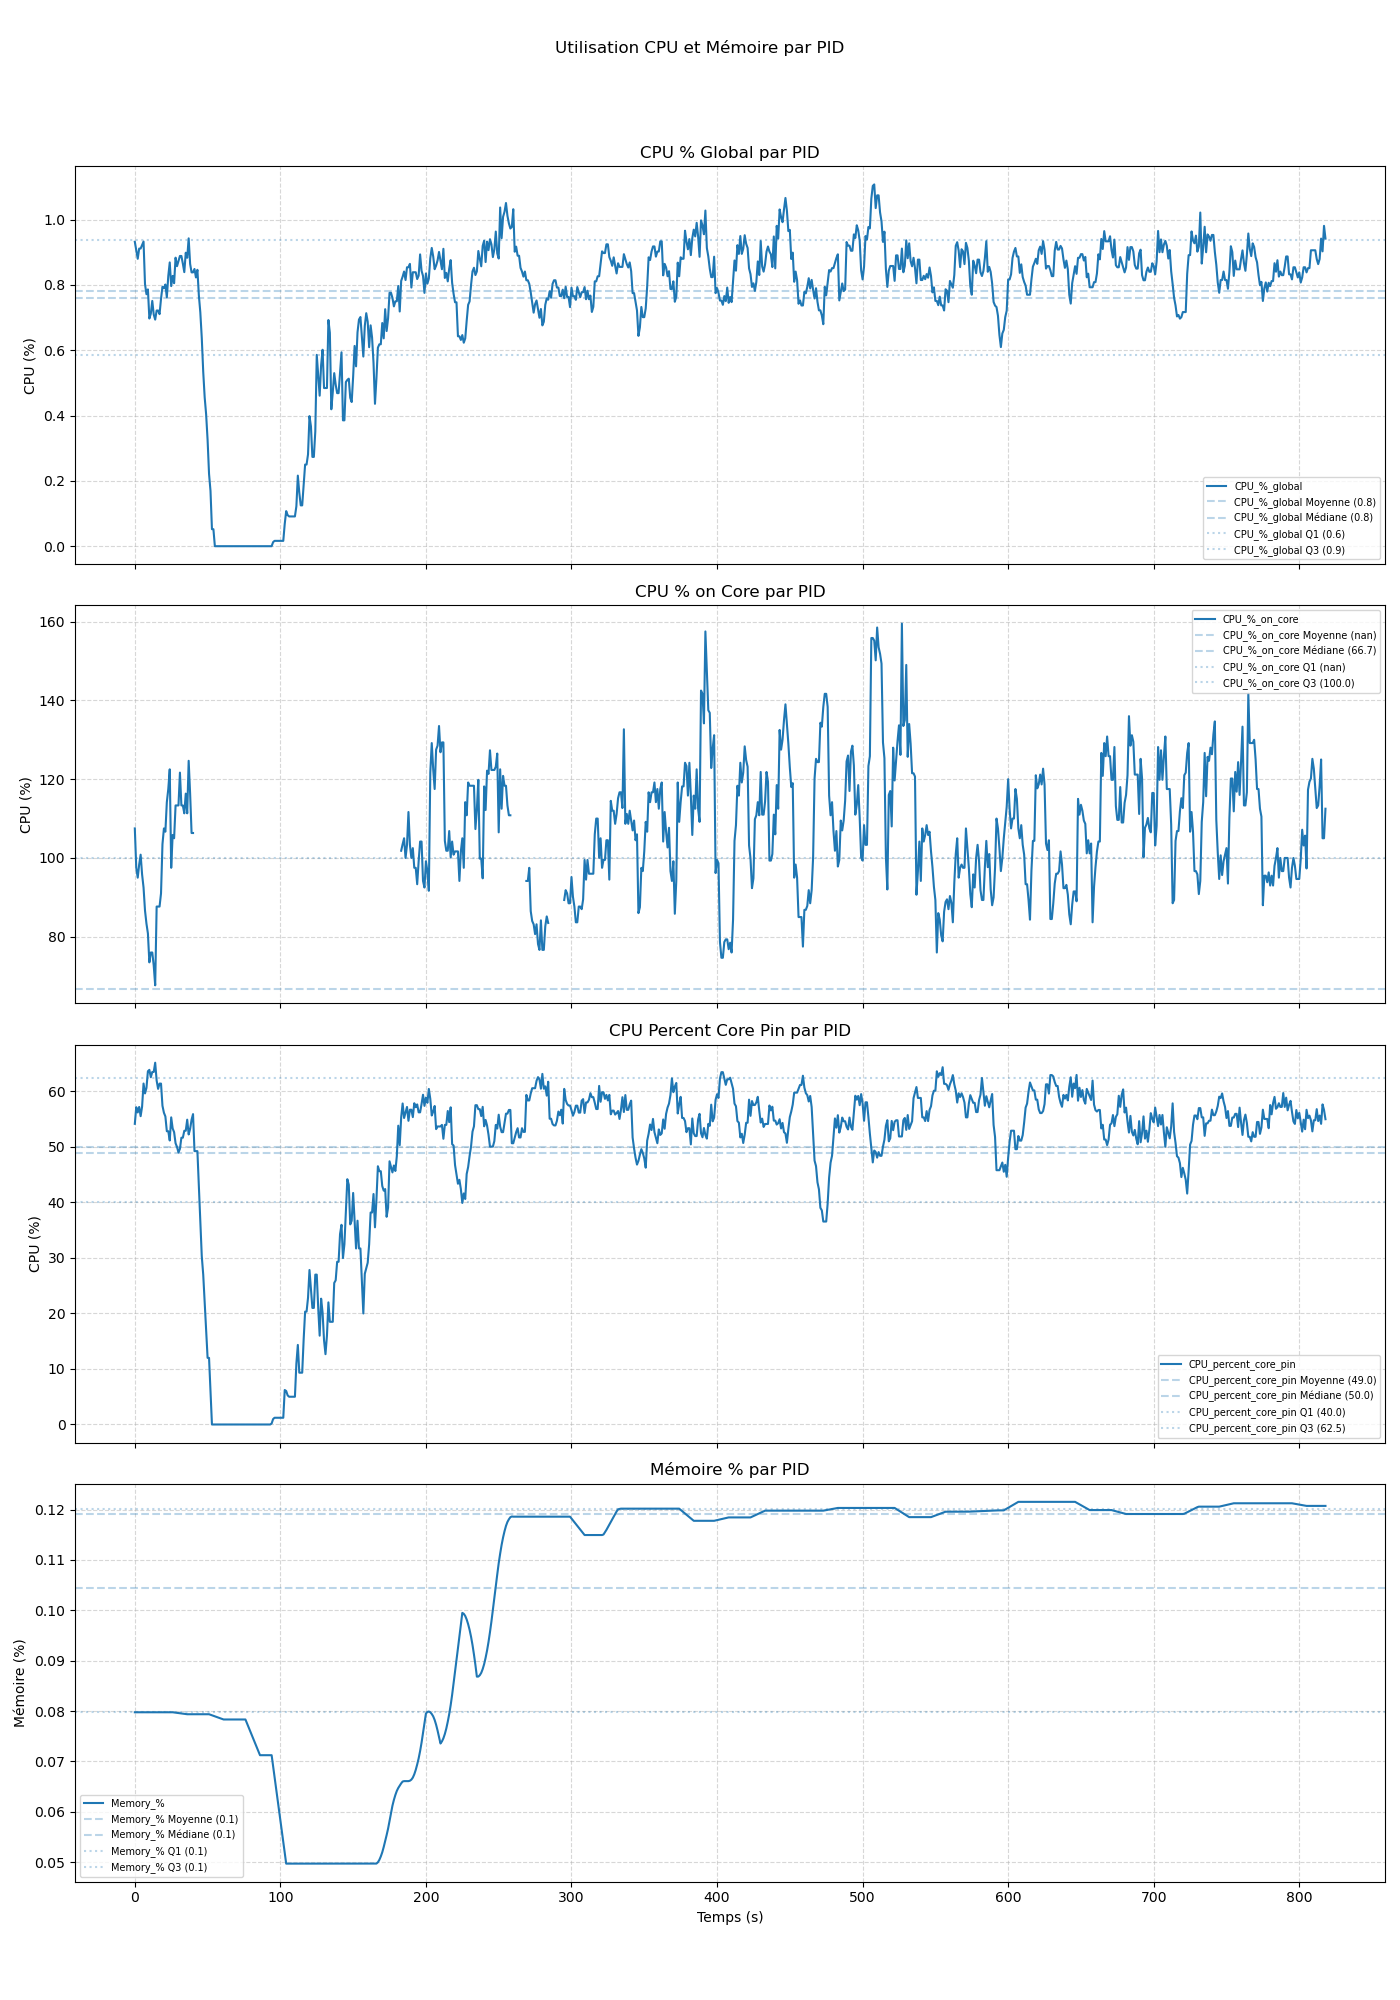
\includegraphics[width=\linewidth]{odb/cpu-conso-BE-128K.png}
                \centering\small Conso BE CPU/RAM ODB (128Ko)
            \end{column}

            \begin{column}{0.48\textwidth}
                
\includegraphics[width=\linewidth]{vanilla/cpu-conso-BE-128K.png}
                \centering\small Conso BE CPU/RAM Vanilla (128Ko)
            \end{column}
        
        \end{columns}
    \end{card}
\end{frame}

\begin{frame}{Temps de réponse moyen, Payload 128Ko}
    \begin{card}
        \begin{columns}

            \begin{column}{0.48\textwidth}
                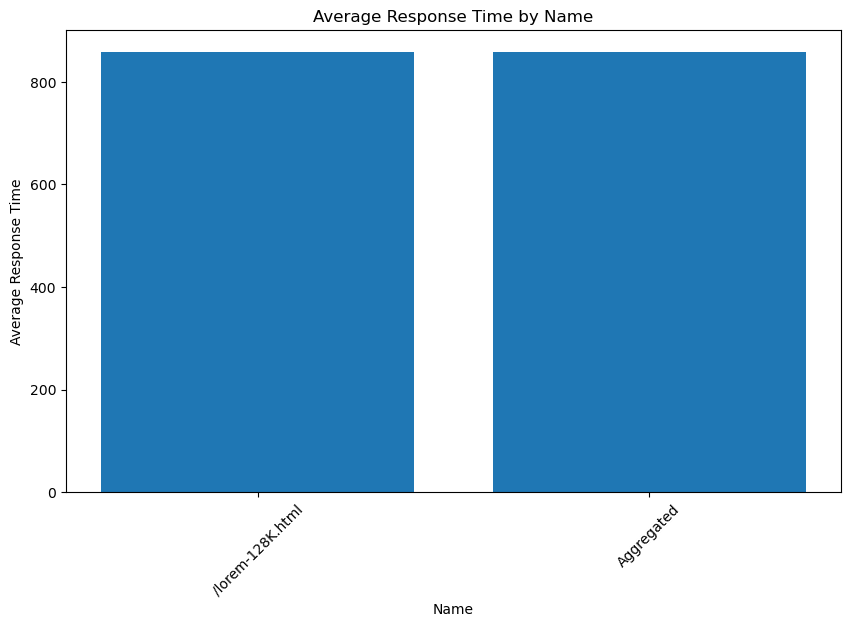
\includegraphics[width=\linewidth]{odb/avg-rtt-128K.png}
                \centering\small Temps de réponse moyen ODB (128Ko)
            \end{column}

            \begin{column}{0.48\textwidth}
                
\includegraphics[width=\linewidth]{vanilla/avg-rtt-128K.png}
                \centering\small Temps de réponse moyen Vanilla (128Ko)
            \end{column}
        
        \end{columns}
    \end{card}
\end{frame}

%%%%%%%%%%%%%%%%%%%%%%%%%%%%%%%%%%%%%%%%%%%%%%%%%
% Consommation CPU et RAM 256Ko
%%%%%%%%%%%%%%%%%%%%%%%%%%%%%%%%%%%%%%%%%%%%%%%%%
\begin{frame}{Consommation CPU et RAM, Payload 256Ko (FE)}
    \begin{card}
        \begin{columns}

            \begin{column}{0.48\textwidth}
                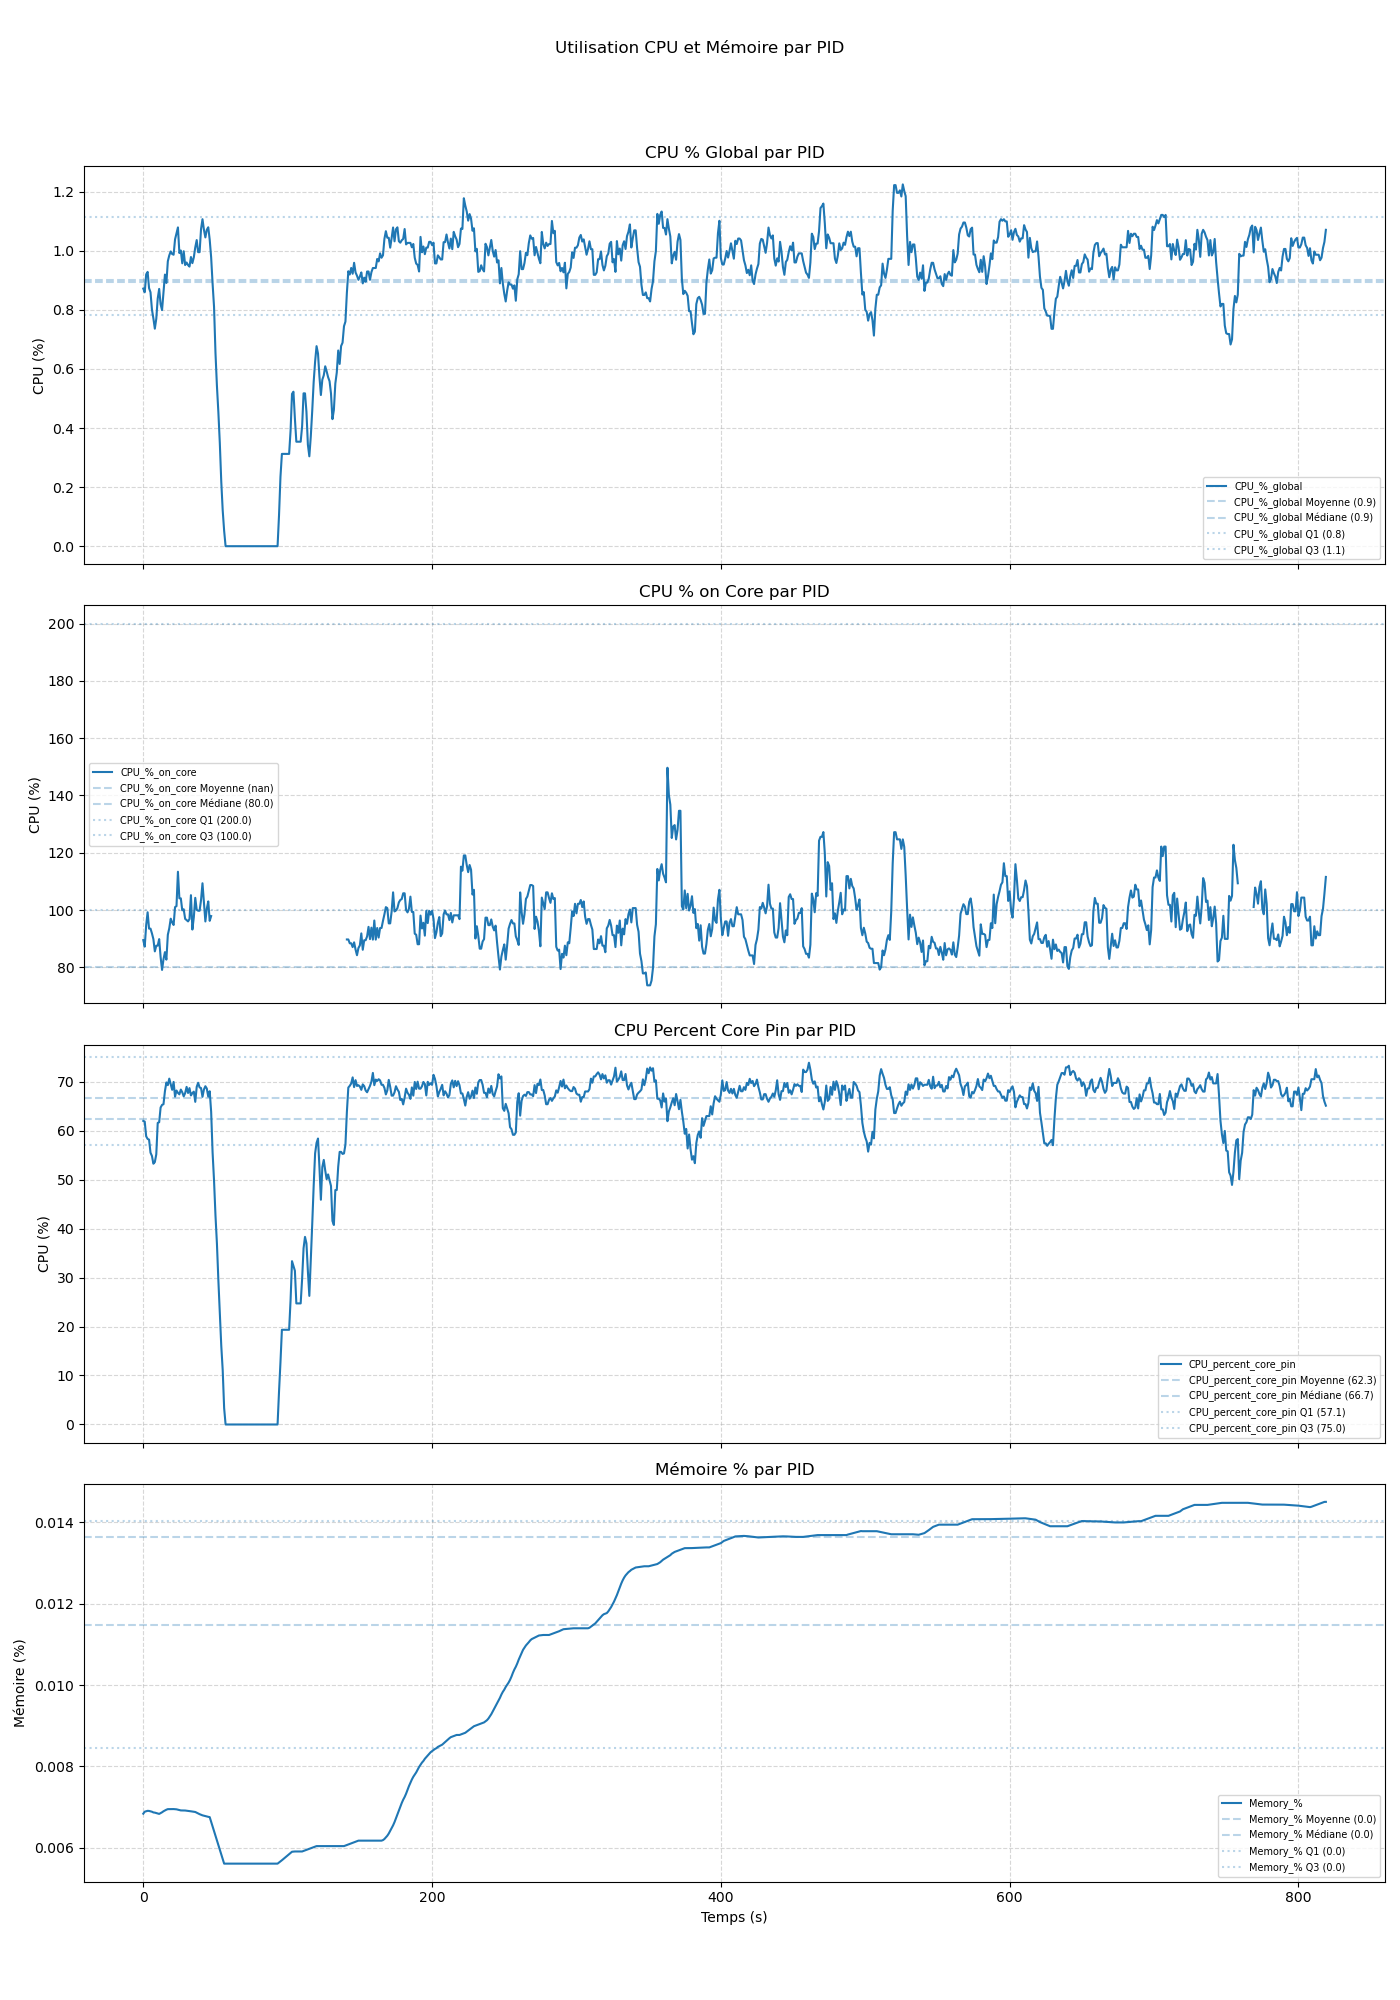
\includegraphics[width=\linewidth]{odb/cpu-conso-FE-256K.png}
                \centering\small Conso FE CPU/RAM ODB (256Ko)
            \end{column}

            \begin{column}{0.48\textwidth}
                
\includegraphics[width=\linewidth]{vanilla/cpu-conso-FE-256K.png}
                \centering\small Conso FE CPU/RAM Vanilla (256Ko)
            \end{column}
        
        \end{columns}
    \end{card}
\end{frame}

\begin{frame}{Consommation CPU et RAM, Payload 256Ko (IS)}
    \begin{card}
        \begin{columns}

            \begin{column}{0.48\textwidth}
                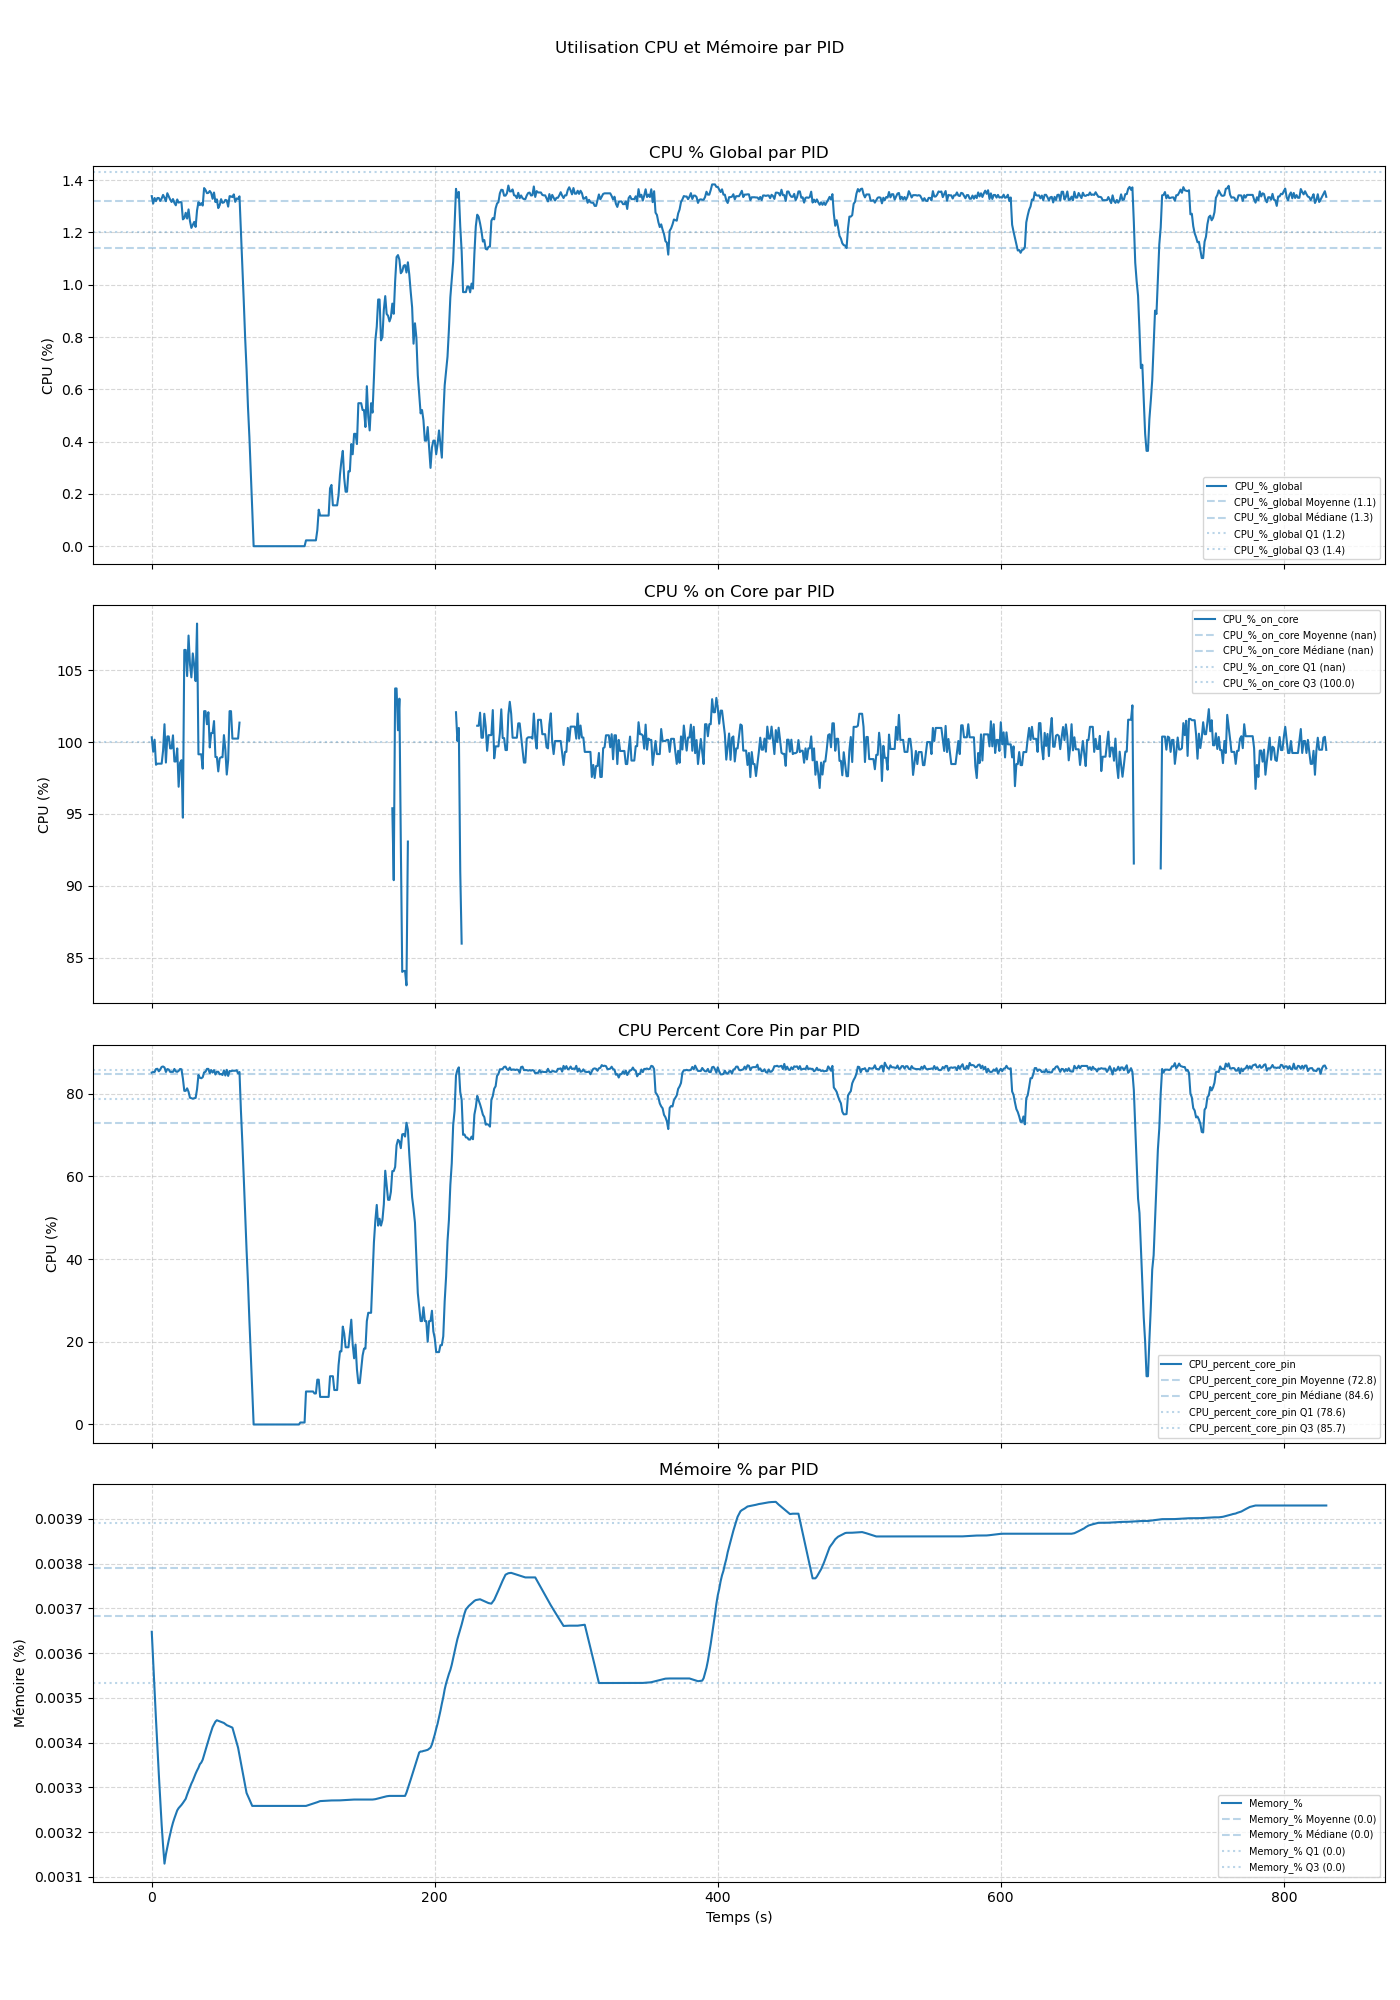
\includegraphics[width=\linewidth]{odb/cpu-conso-IS-256K.png}
                \centering\small Conso IS CPU/RAM ODB (256Ko)
            \end{column}

            \begin{column}{0.48\textwidth}
                
\includegraphics[width=\linewidth]{vanilla/cpu-conso-IS-256K.png}
                \centering\small Conso IS CPU/RAM Vanilla (256Ko)
            \end{column}
        
        \end{columns}
    \end{card}
\end{frame}

\begin{frame}{Consommation CPU et RAM, Payload 256Ko (BE)}
    \begin{card}
        \begin{columns}

            \begin{column}{0.48\textwidth}
                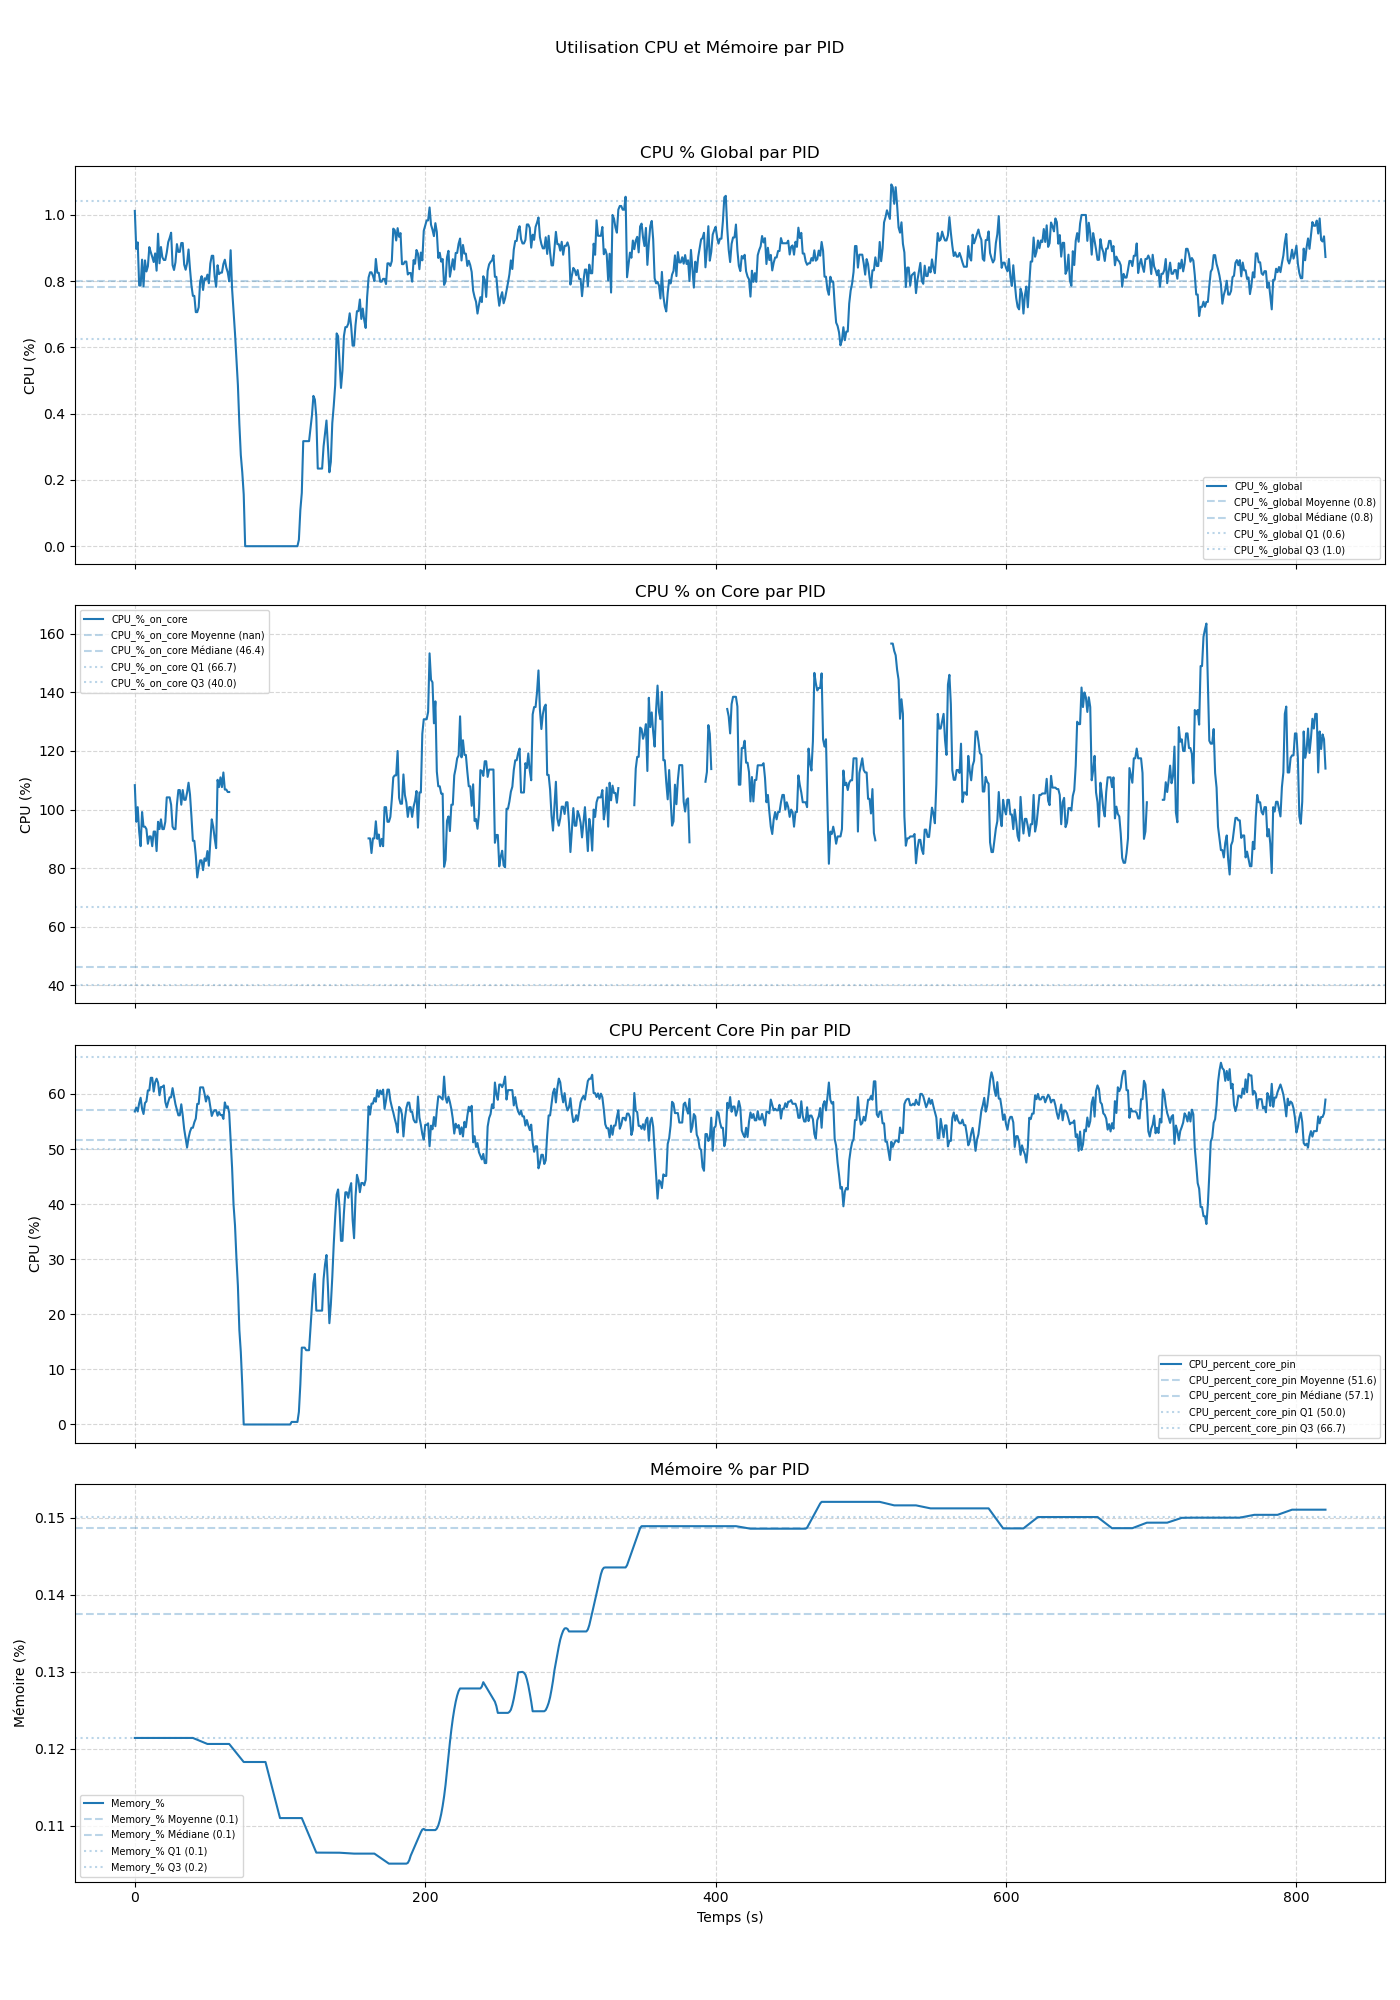
\includegraphics[width=\linewidth]{odb/cpu-conso-BE-256K.png}
                \centering\small Conso BE CPU/RAM ODB (256Ko)
            \end{column}

            \begin{column}{0.48\textwidth}
                
\includegraphics[width=\linewidth]{vanilla/cpu-conso-BE-256K.png}
                \centering\small Conso BE CPU/RAM Vanilla (256Ko)
            \end{column}
        
        \end{columns}
    \end{card}
\end{frame}

\begin{frame}{Temps de réponse moyen, Payload 256Ko}
    \begin{card}
        \begin{columns}

            \begin{column}{0.48\textwidth}
                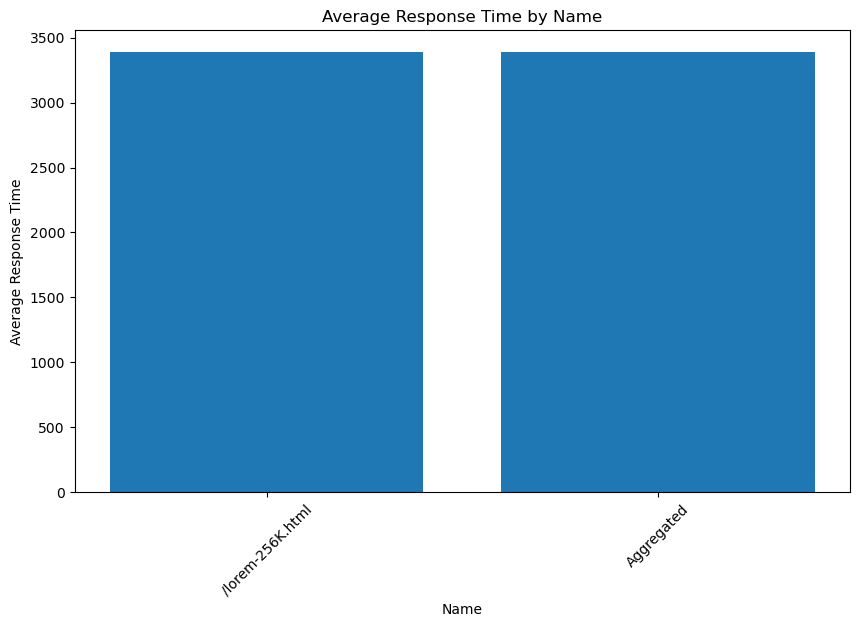
\includegraphics[width=\linewidth]{odb/avg-rtt-256K.png}
                \centering\small Temps de réponse moyen ODB (256Ko)
            \end{column}

            \begin{column}{0.48\textwidth}
                
\includegraphics[width=\linewidth]{vanilla/avg-rtt-256K.png}
                \centering\small Temps de réponse moyen Vanilla (256Ko)
            \end{column}
        
        \end{columns}
    \end{card}
\end{frame}


\begin{frame}{Explications possible de la réduction de performance }
\begin{card}
	\begin{itemize}
		\item  Modification du buffer RX/TX tcp à 65536 octets (éventuellement trop petit à partir de 128Ko de payload)
		\item  Utilisation de Hashmaps pour stocker les connexions, les buffers virtuels,etc..
		\item  Induit l'utilisation de verrous qui peuvent introduire de la latence en cas de concurrence
		\item  Réalisation teechnique d'ODB et des test différents de la thèse de Brice (peut-être plus de charge ici)
		\item  Utilisation de socket bloquante pour l'accès à la Remote Access Memory du back-end
	\end{itemize}
\end{card}
\end{frame}



\end{document}